\section{Results and Discussion}
\label{ch1:sec:results-and-discussion}

In this section, all results are presented and briefly discussed.
Each of the three assessments in this section focuses on improvements in voltage level, improvements in network efficiency (i.e. power quality and network losses), and improvements in resource utilisation.
Hence, only a subset of all results is included, but the complete set of results has been appended to this Thesis in Appendix \ref{appx-a:ch1}.

\subsection{Time Series Analysis}
\label{ch1:subsec:time-series-analysis}

The ESMU's largest impact on network voltage levels can be noticed at the ESMU's PCC.
Consequently, any adjustments to the ESMU powers should become most noticeable, too.
This impact can clearly be observed in Figure \ref{ch1:fig:ts-esmu-voltages}.

\begin{figure}\centering
	\subfloat[Voltage levels at ESMU's PCC when minimising its voltage deviation \hl{(nominal substation voltage is 252V)}]{%
		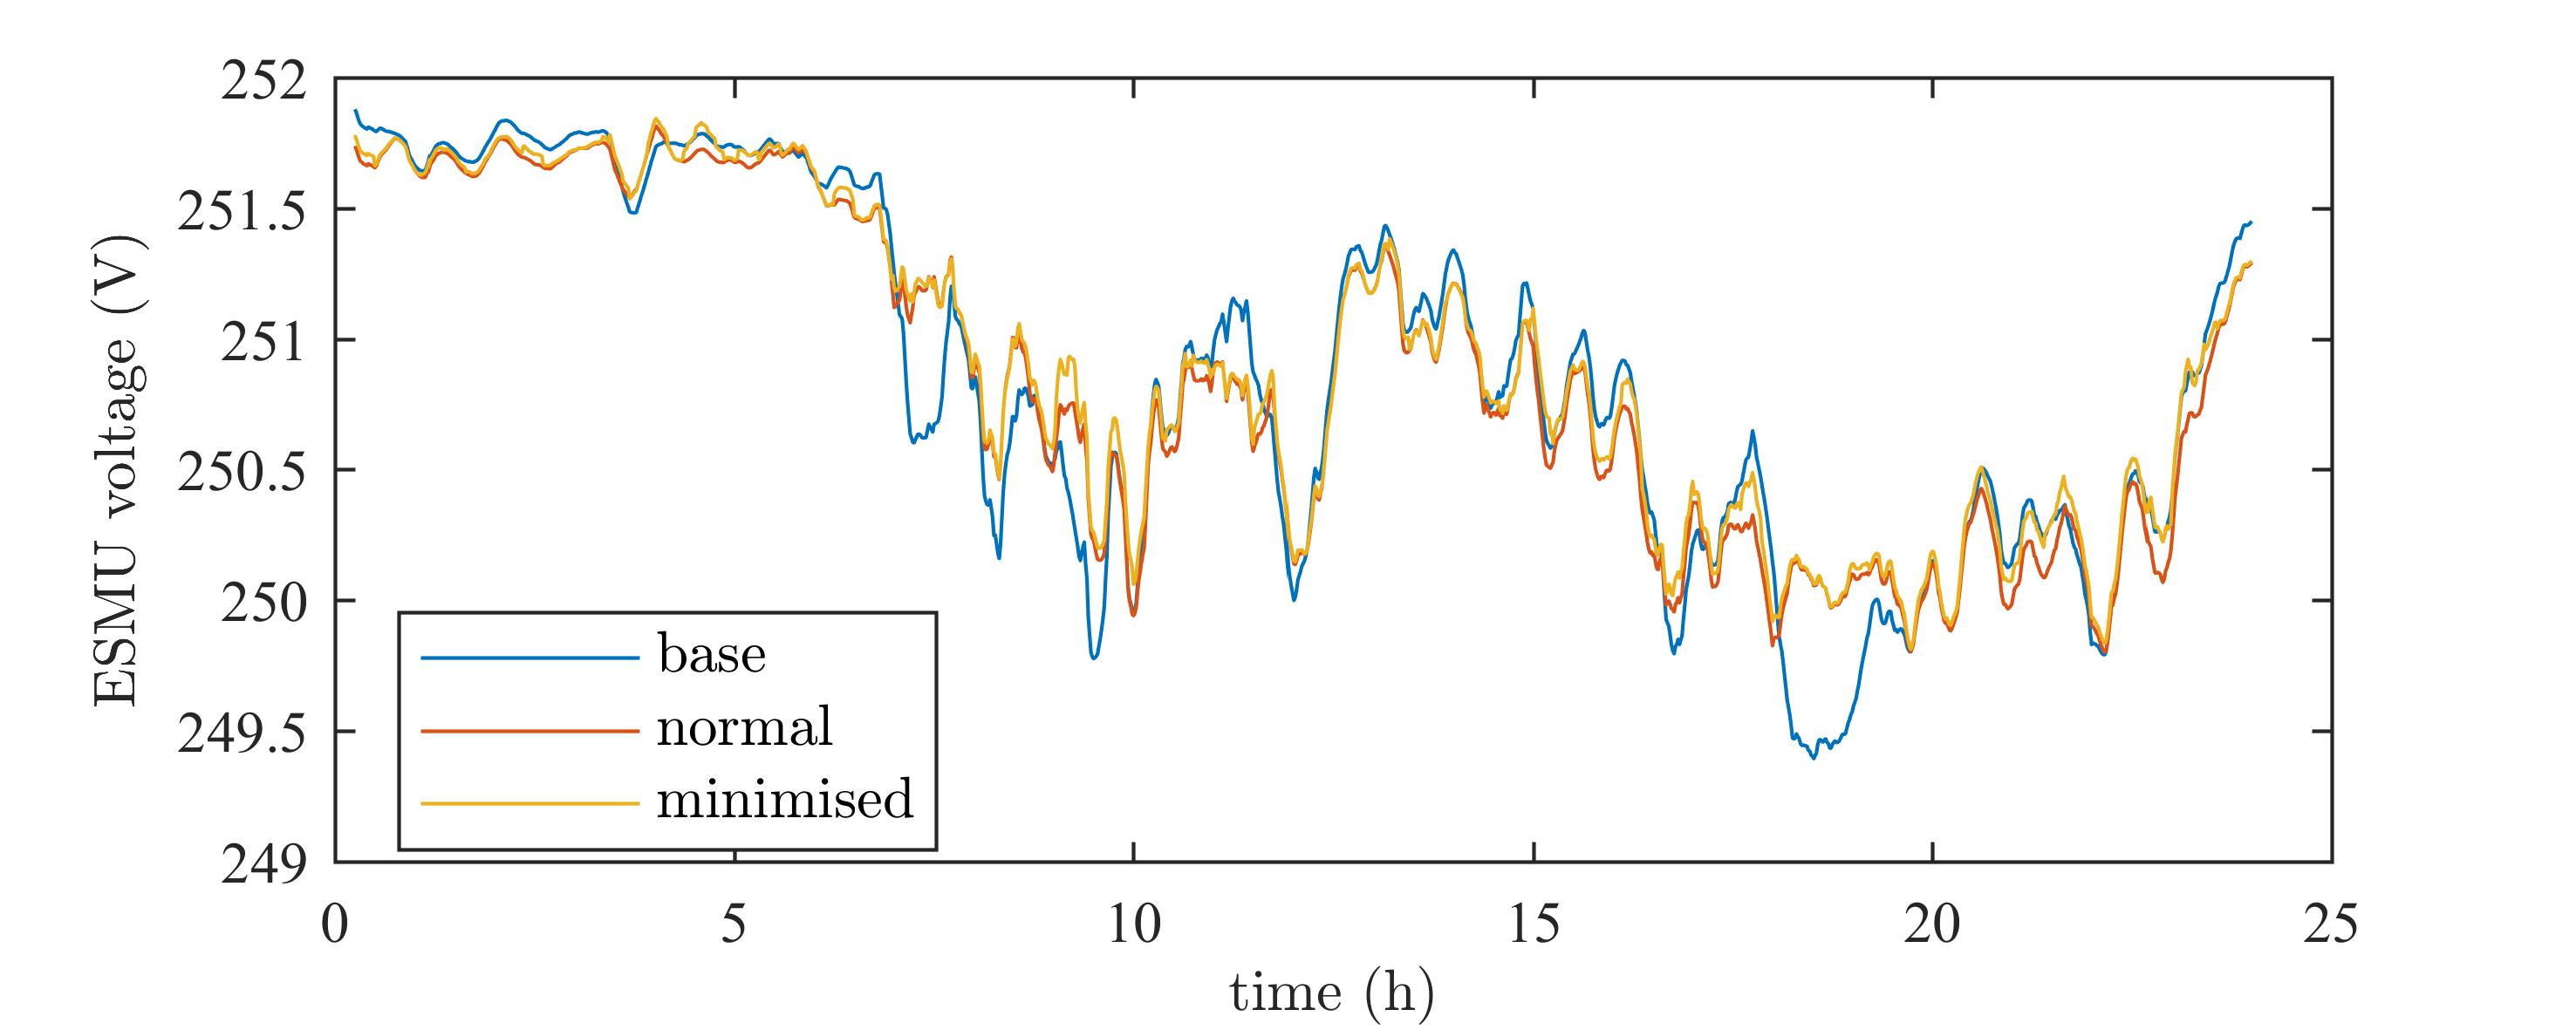
\includegraphics{_chapter1/fig/results/ts-esmu-voltages_}%
		\label{ch1:subfig:ts-esmu-voltage}%
	}\\
%	\vspace{5mm}
	\subfloat[Cost associated with the minimisation of the ESMU's PCC voltage deviation]{%
		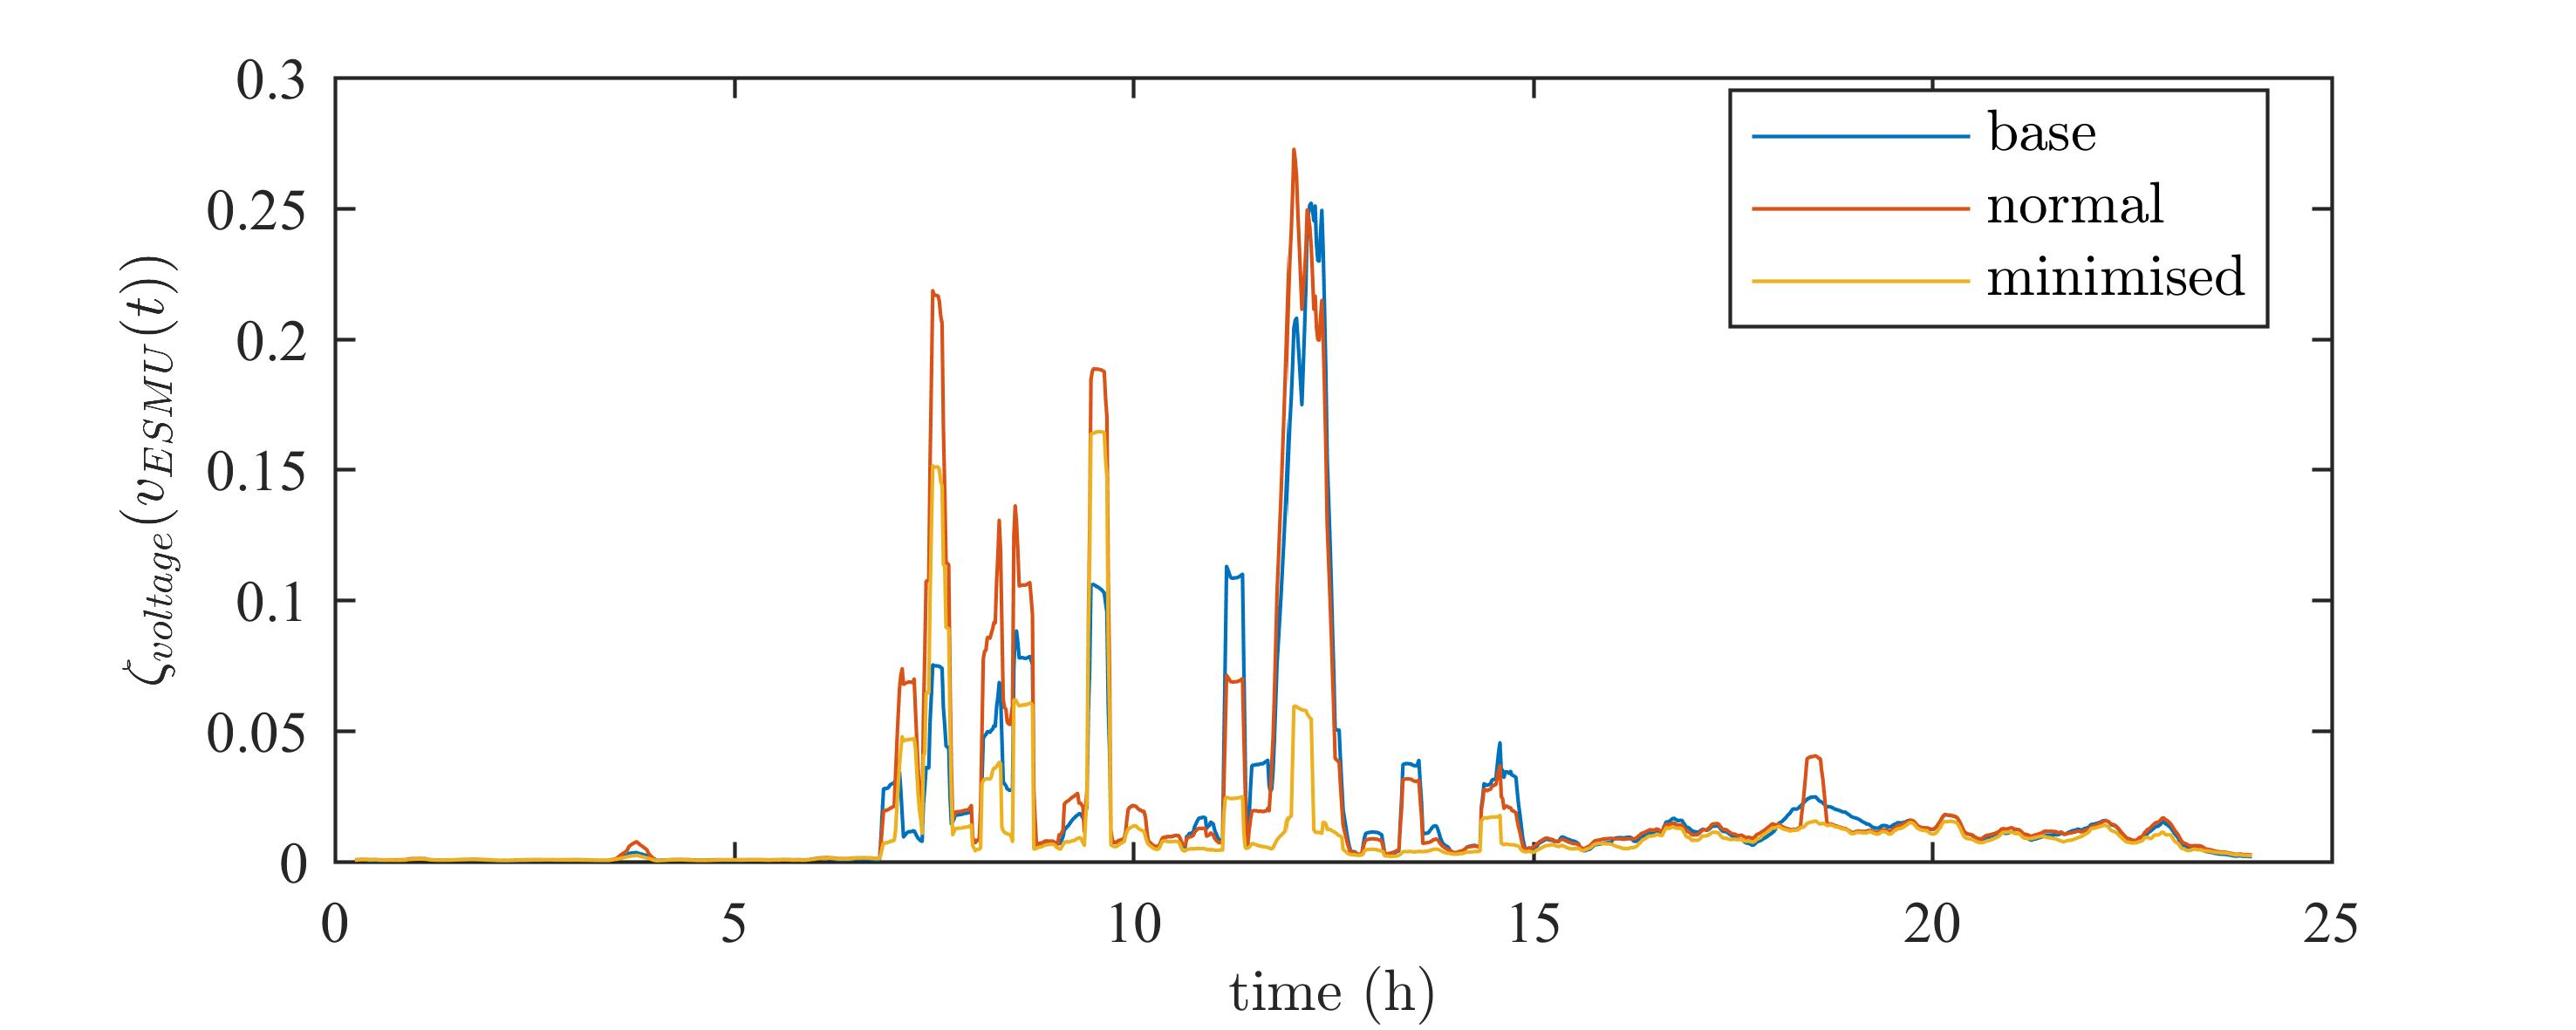
\includegraphics{_chapter1/fig/results/ts-esmu-voltages}%
		\label{ch1:subfig:ts-esmu-voltage-cost}%
	}
\caption{Voltage level modifications as noted at the ESMU's PCC by adjusting its schedule}
\label{ch1:fig:ts-esmu-voltages}
\end{figure}

In this figure, the \textit{base} and \textit{normal} case's voltage profiles are plotted alongside the \textit{minimisation} case, for which voltage deviation is minimised.
The plot shows that during the night's light load (i.e. from 0:00 to 6:00), ESMU was able to boost its voltage towards the nominal feeder voltage.
This is also the case during the lighter load in the afternoon (i.e. between 12:00-14:00).
But during the rest of the day when network load increases, the ESMU is unable to reduce voltage deviation to match its PCC voltage with the network's nominal substation voltage.
The reason behind this behaviour that the ESMU has allocated its resources to serve for the underlying half-hourly ESMU schedule.
Therefore, the remaining resources that could provide voltage support during periods of low demand become limited during periods of high demand.
Combined with the fact that the LV distribution network is more resistive than inductive (i.e. unlike HV transmission networks), reactive power injection to support voltage levels has a reduced impact.
Nonetheless, due to the constant yet small availability of power resources, the ESMU was able to boost voltages by to some extent at all times; this can be seen in Figure \ref{ch1:subfig:ts-esmu-voltage-cost}, where the associated cost has always been reduced in comparison to the base and normal.

The ability to support voltage levels at the ESMU's PCC is interesting, yet to support voltage levels at all buses throughout the network is more relevant, since some of these buses are linked to customers, for which maintaining a constant voltage level is essential.
Therefore, the next voltage plot inspects both the highest and lowest voltage level that was recorded throughout the network.

\begin{figure}\centering
	\subfloat[Highest and lowest voltage levels that were recorded throughout the network when minimising the worst voltage deviation \hl{(nominal substation voltage is 252V)}]{%
		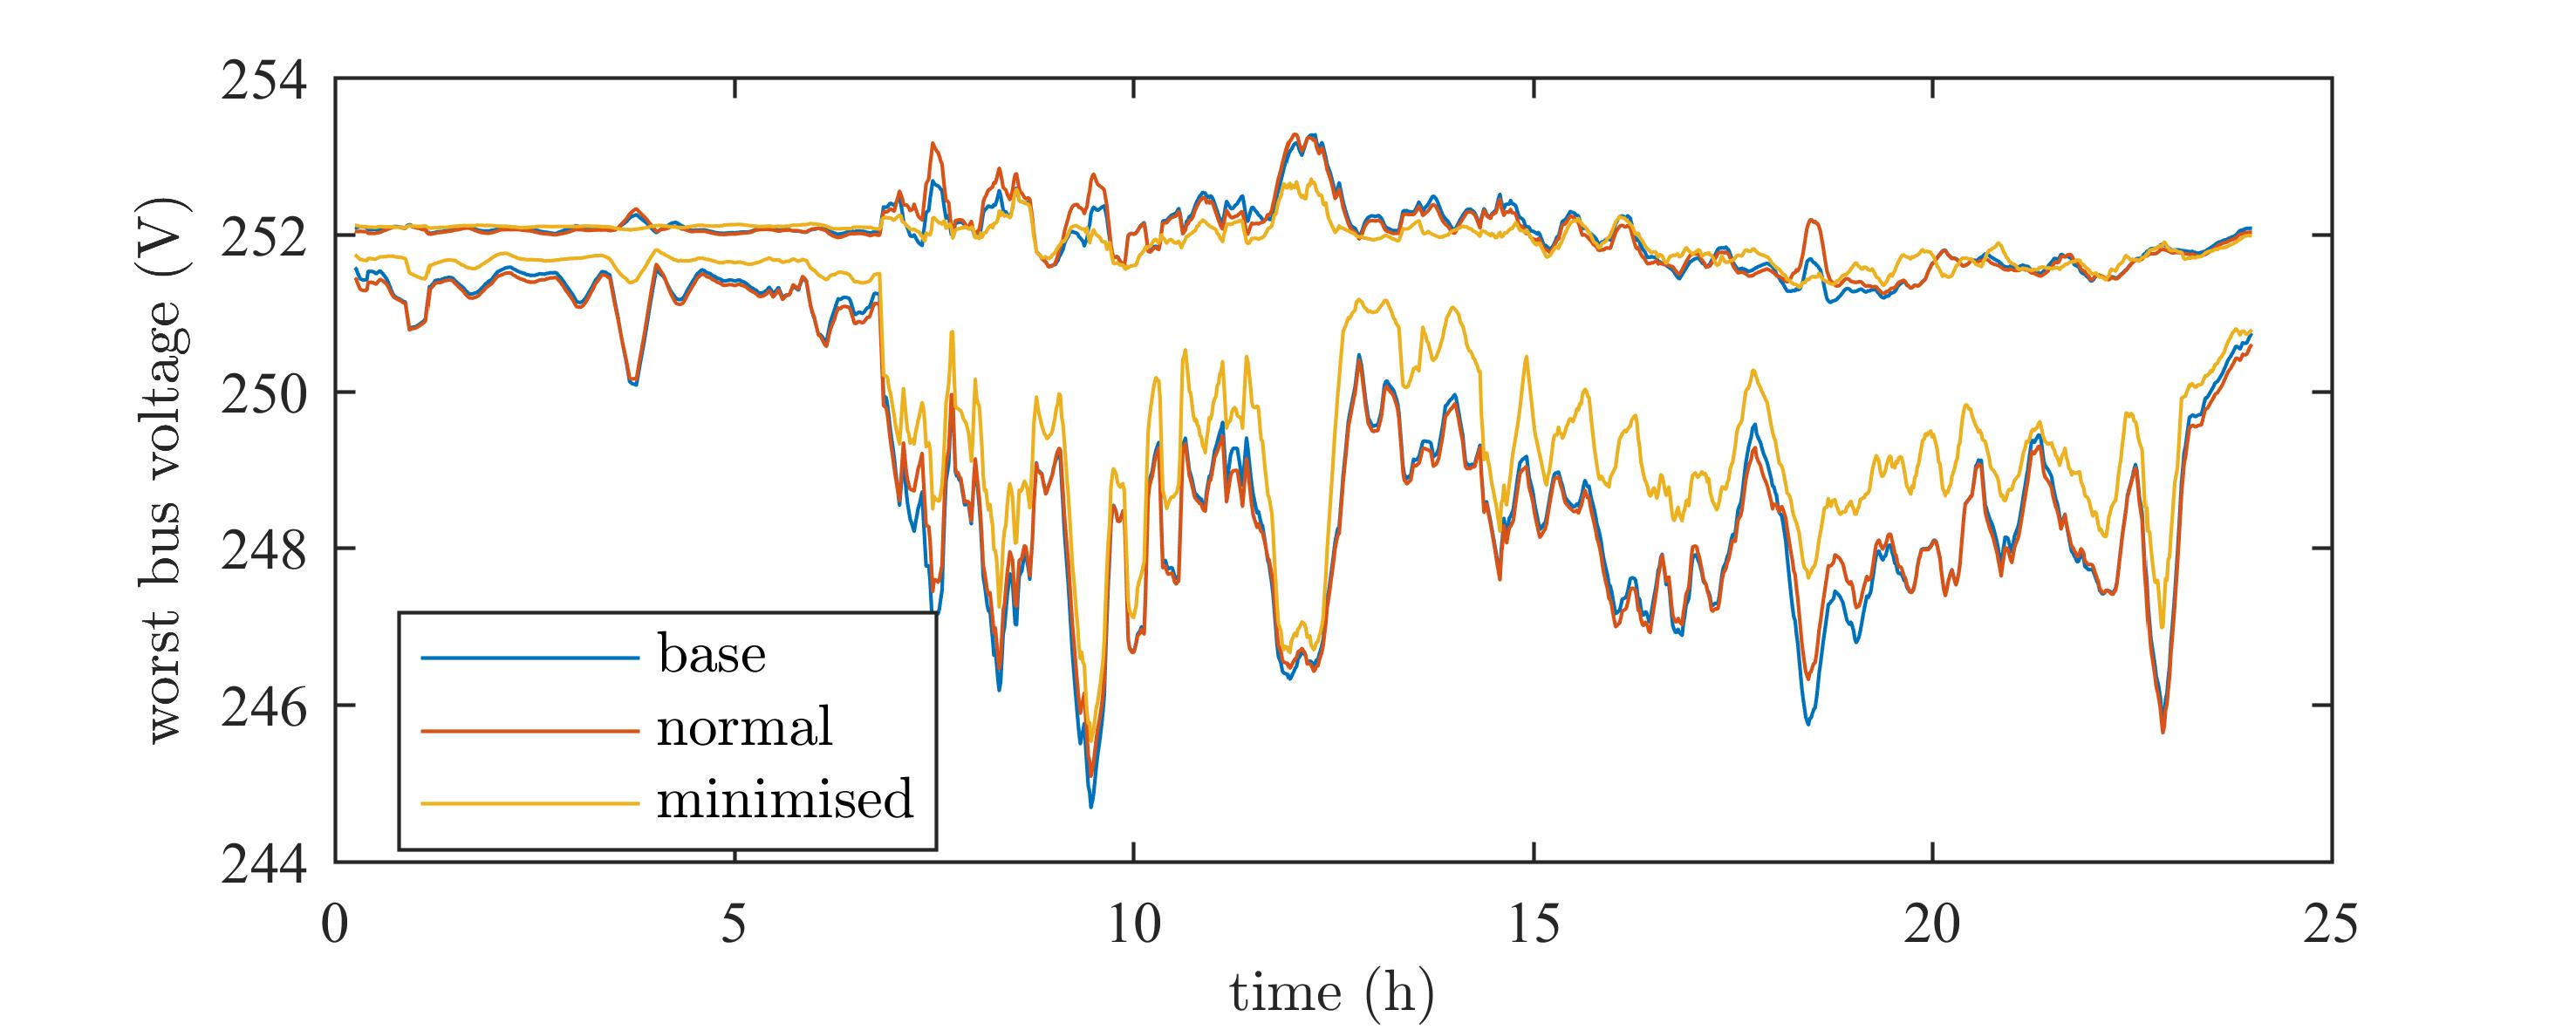
\includegraphics{_chapter1/fig/results/ts-all-voltages_}%
		\label{ch1:subfig:ts-all-voltages}%
	}\\
%	\vspace{5mm}
	\subfloat[Cost associated with the worst voltage deviation throughout the entire network]{%
		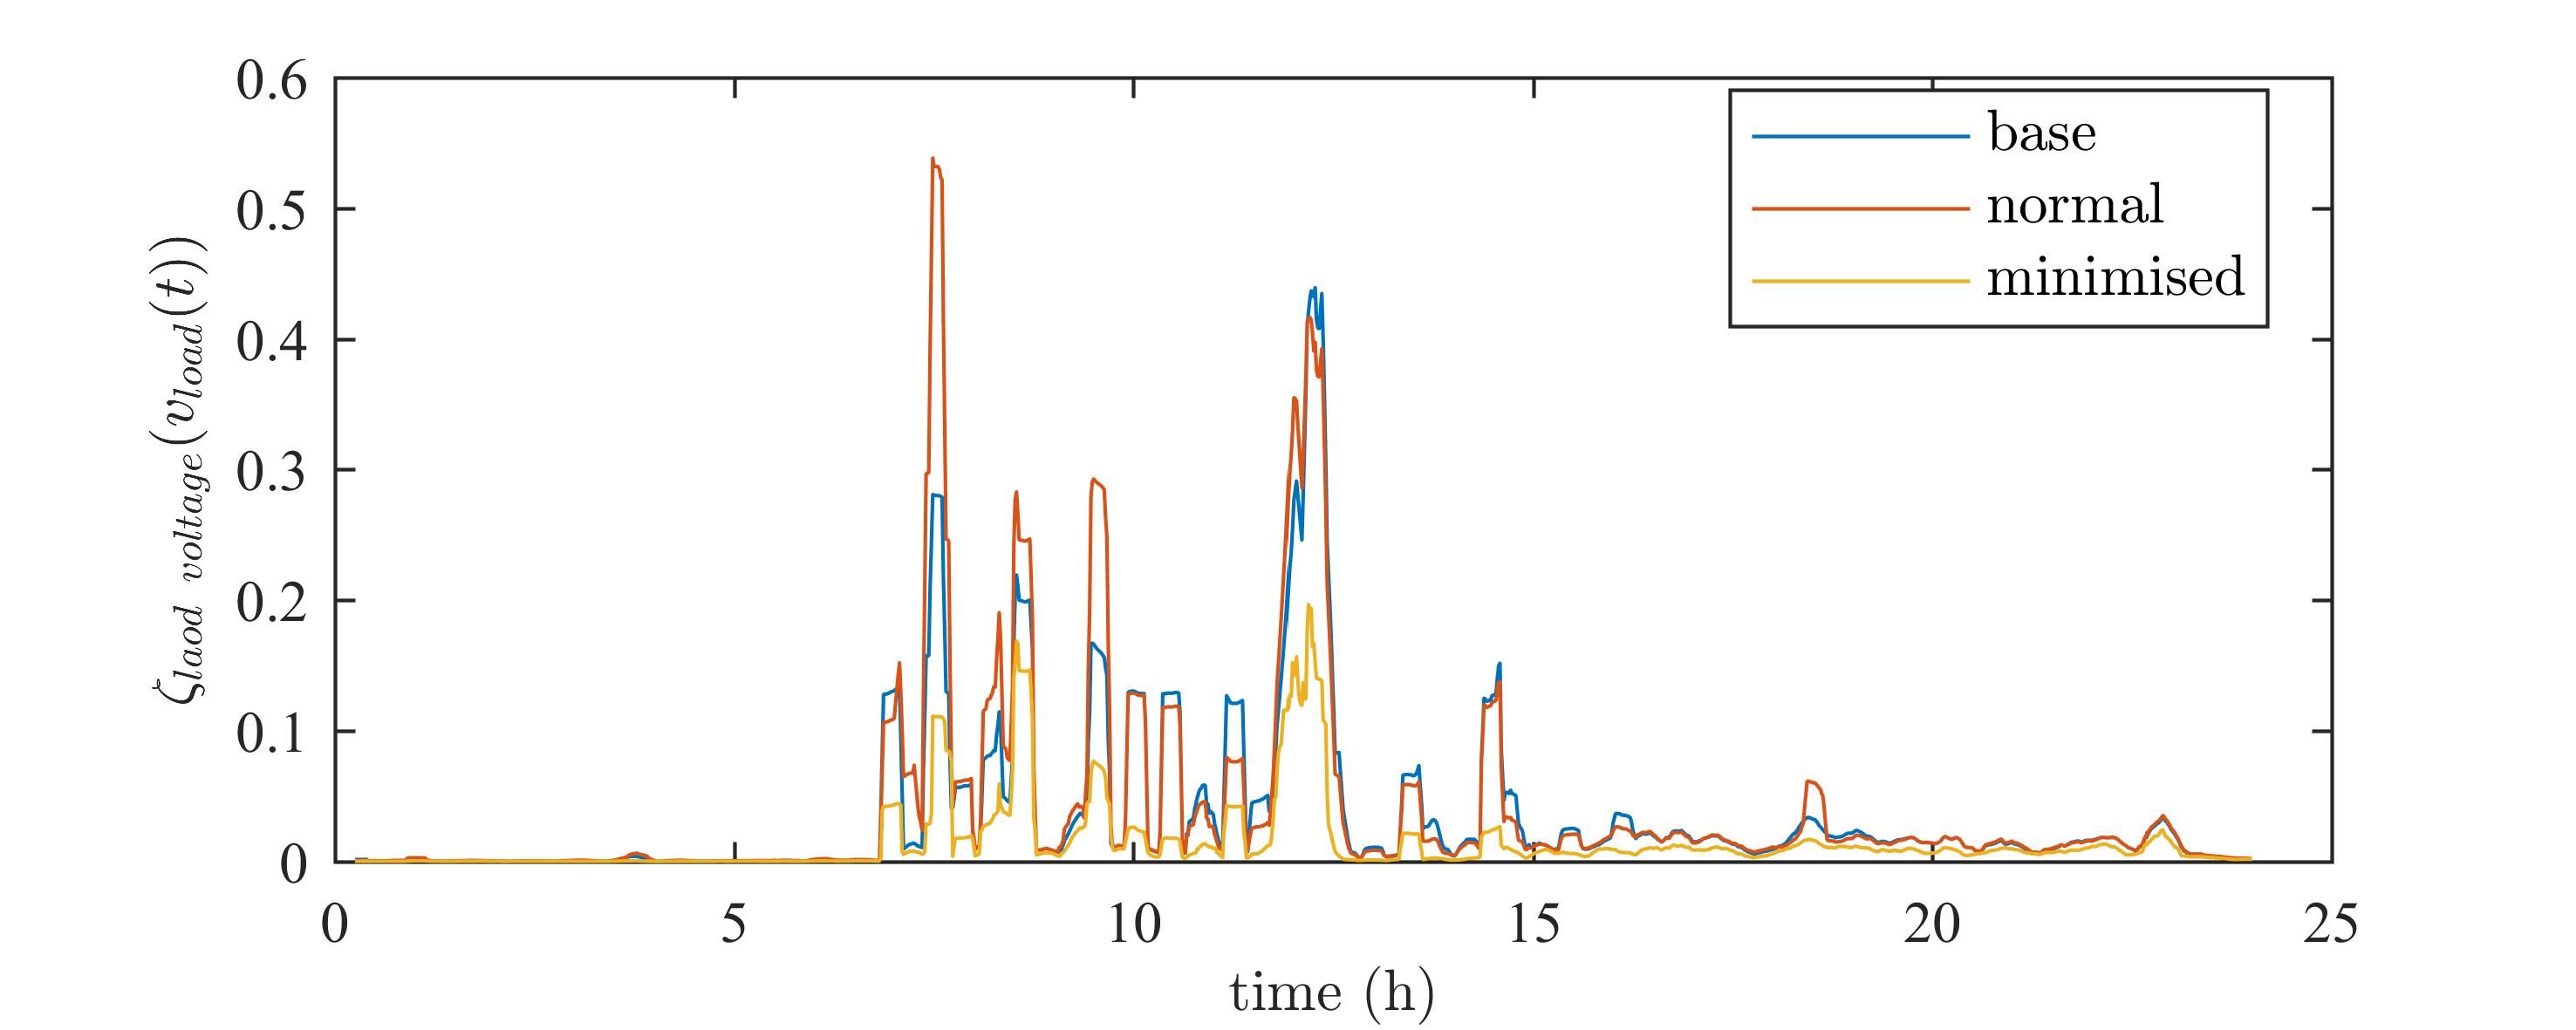
\includegraphics{_chapter1/fig/results/ts-all-voltages}%
		\label{ch1:subfig:ts-all-voltages-cost}%
	}
\caption{Voltage level improvements at all buses in the entire distribution network due to the ESMU schedule adjustment.}
\label{ch1:fig:ts-all-voltages}
\end{figure}

In Figure \ref{ch1:subfig:ts-all-voltages}, despite no voltage violations taking place due to the already boosted substation voltage, the ESMU's positive impact can be observed.
Here, the difference between highest and lowest voltage in the network was noticeably reduced at all times and their average was brought closer to the network's nominal voltage.
The ESMU's function to support the network in providing more stable voltage levels at customer endpoints can therefore be fulfilled.
This fact is also reflected in the associated cost plot, i.e. in Figure \ref{ch1:subfig:ts-all-voltages-cost}.

Beside providing stable voltage levels, power quality should also be upheld to assure that the distribution network operates as efficient as possible.
The first power related parameter that to indicate network efficiency is the phase unbalance.

\begin{figure}\centering
	\subfloat[Network's highest and lowest phase power demand when phase unbalance was minimised]{%
		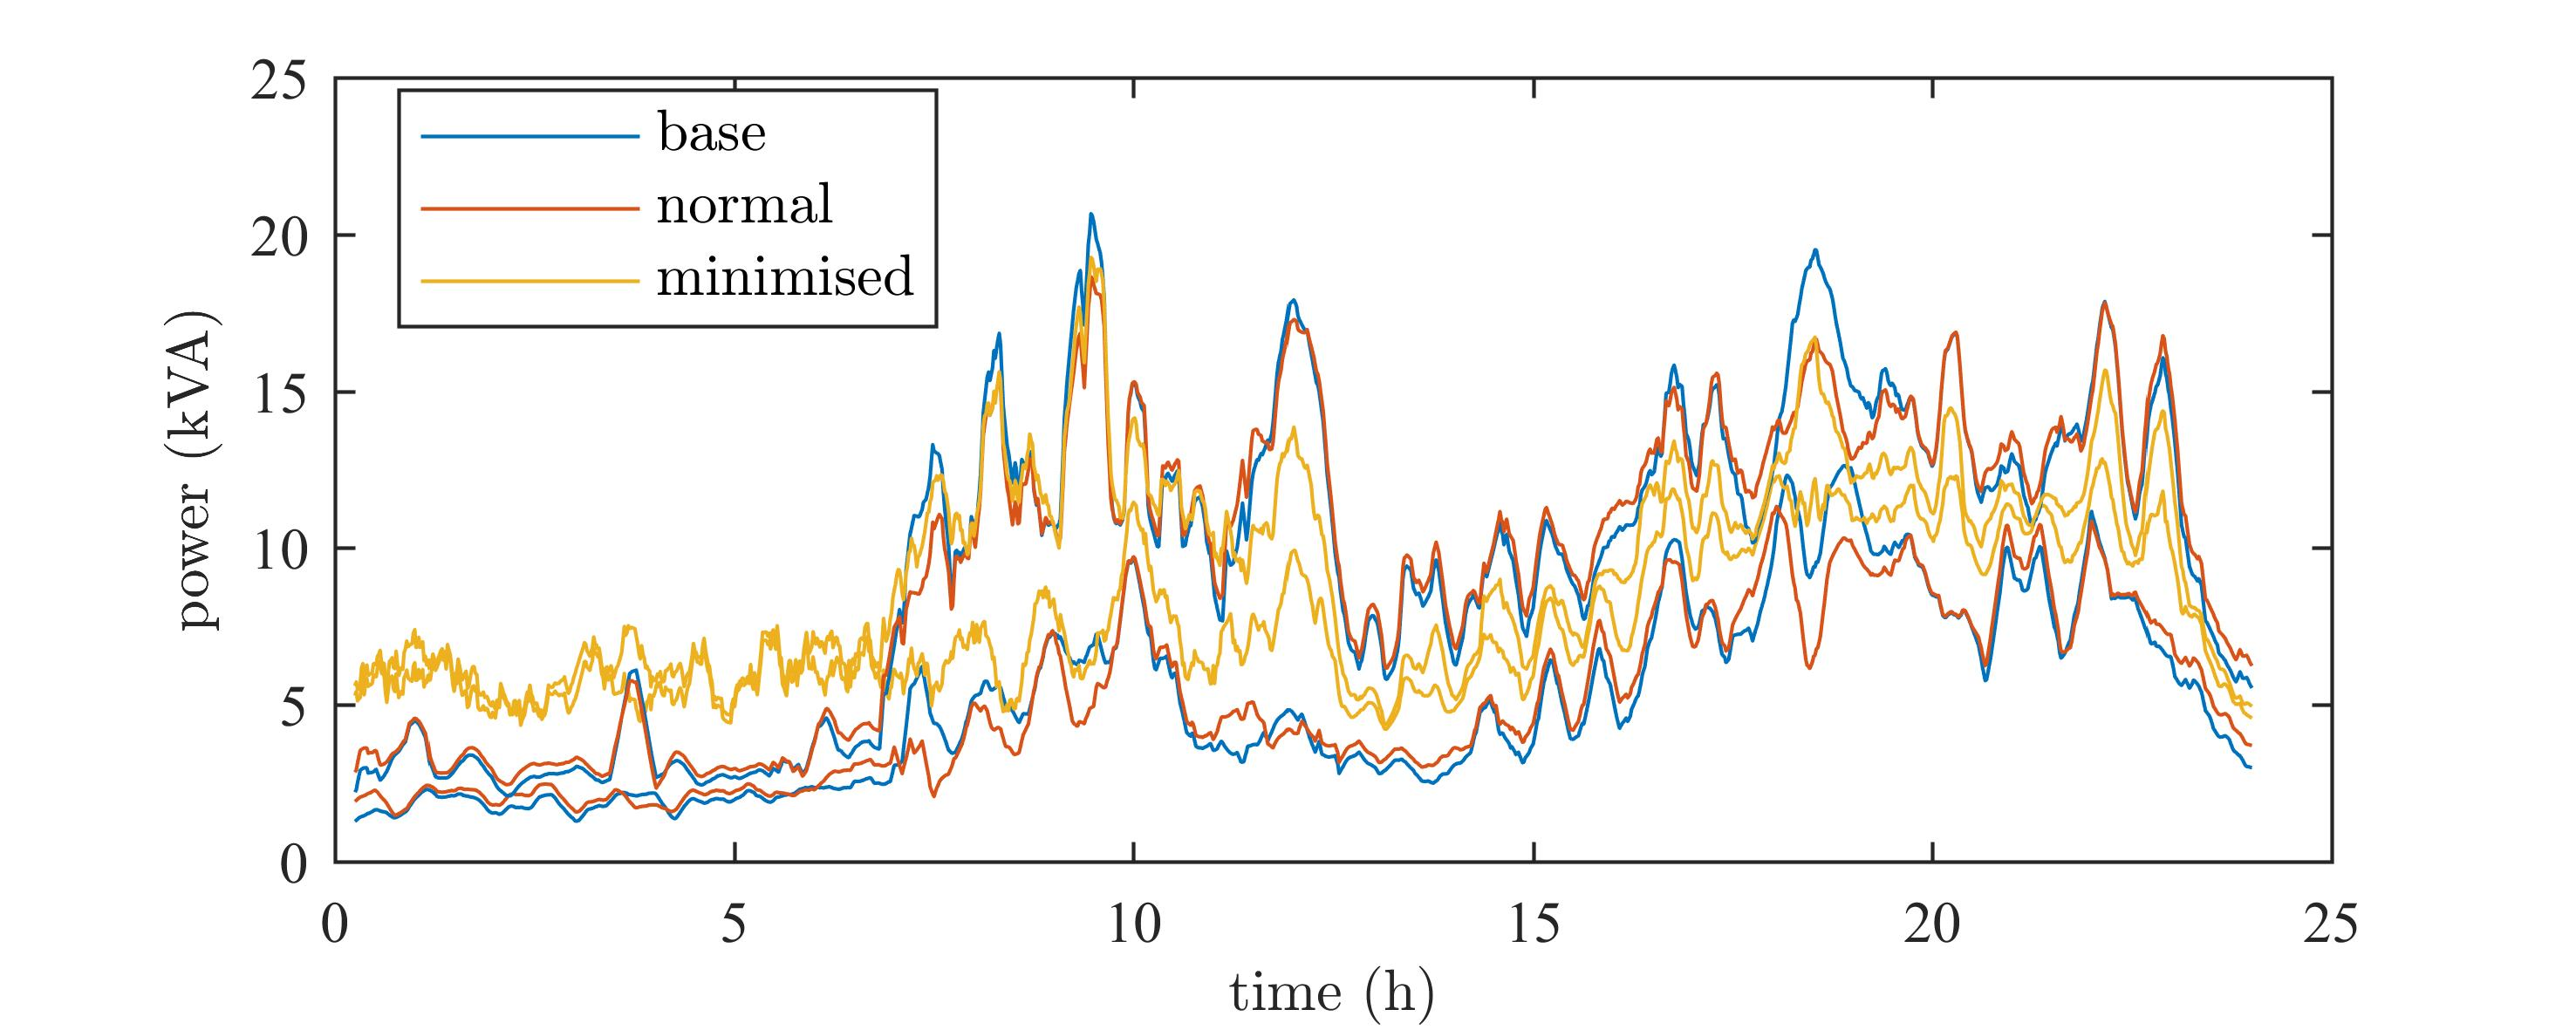
\includegraphics{_chapter1/fig/results/ts-phase-unbalance_}%
		\label{ch1:subfig:ts-phase-unbalance}%
	}\\
%	\vspace{5mm}
	\subfloat[Cost associated with the network's phase unbalance]{%
		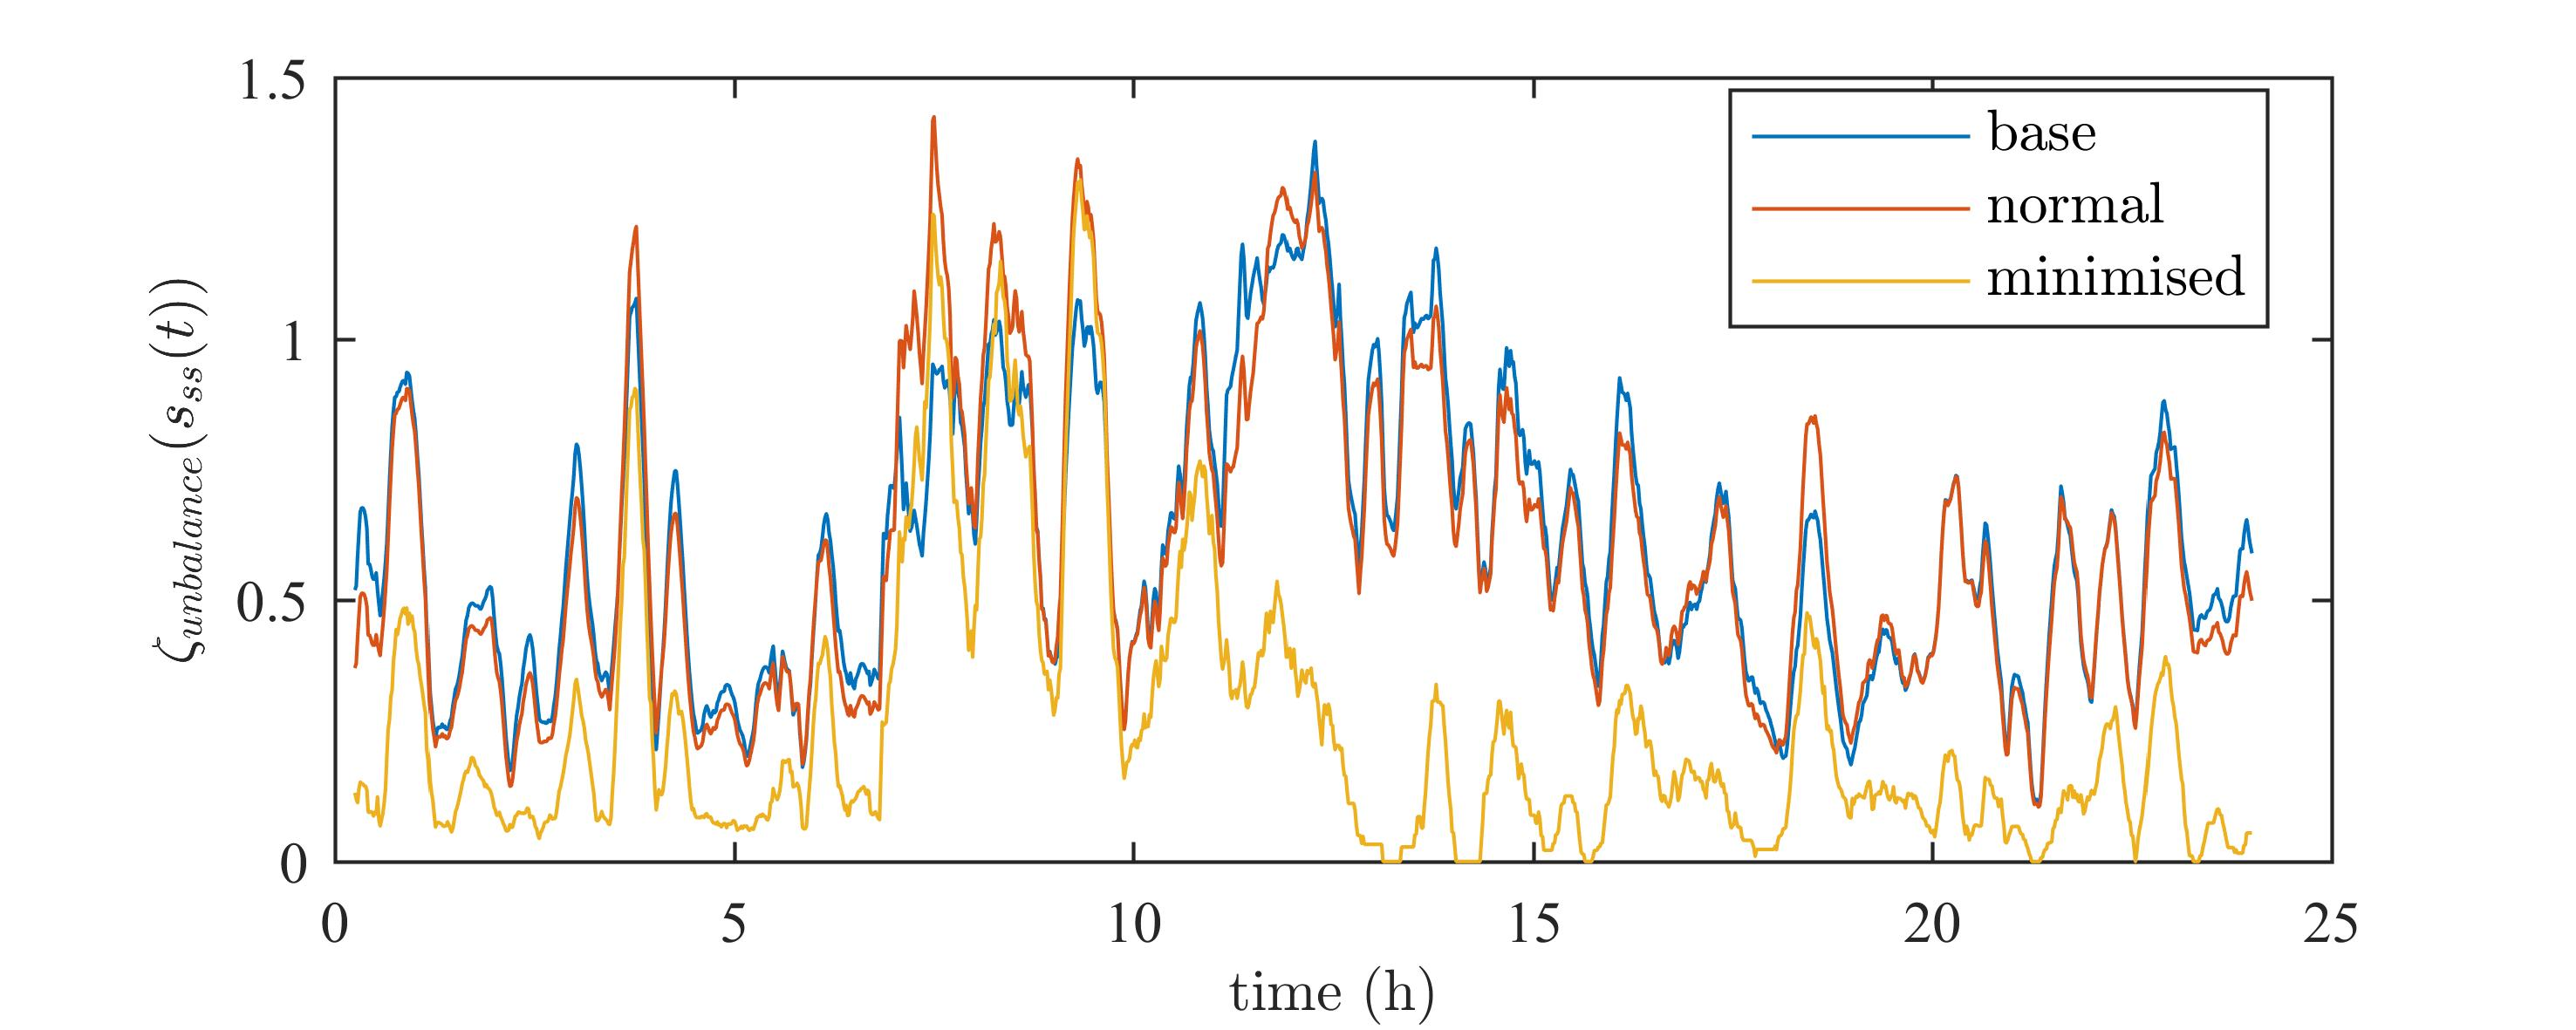
\includegraphics{_chapter1/fig/results/ts-phase-unbalance}%
		\label{ch1:subfig:ts-phase-unbalance-cost}%
	}
\caption{Reduction of the network's phase unbalance due to the adjustment of the ESMU schedule.}
\label{ch1:fig:ts-phase-unbalance}
\end{figure}

In Figure \ref{ch1:subfig:ts-phase-unbalance}, the most and least loaded phases' power values are plotted against time.
At all times, the sub-half-hourly adjustments of the ESMU's schedule could reduce the underlying phase imbalance.
It did so by alleviate some load from the most loaded phase and utilise the unused capacity on the lighter loaded phases.
Correspondingly, the associated phase unbalance cost has noticeably lowered in comparison to the normal and base cases.
It should however be noted, that phase balancing behaviour during the morning hours is predominantly comprised of reactive power injection and absorption, since the ESMU's half-hourly.
Therefore, the tradeoff between adding additional strain on the network, versus balancing phases has to be taken into account.
One unnecessary strain on the network is additional neutral power flow, which is inadvertently linked to phase unbalance.

\begin{figure}\centering
	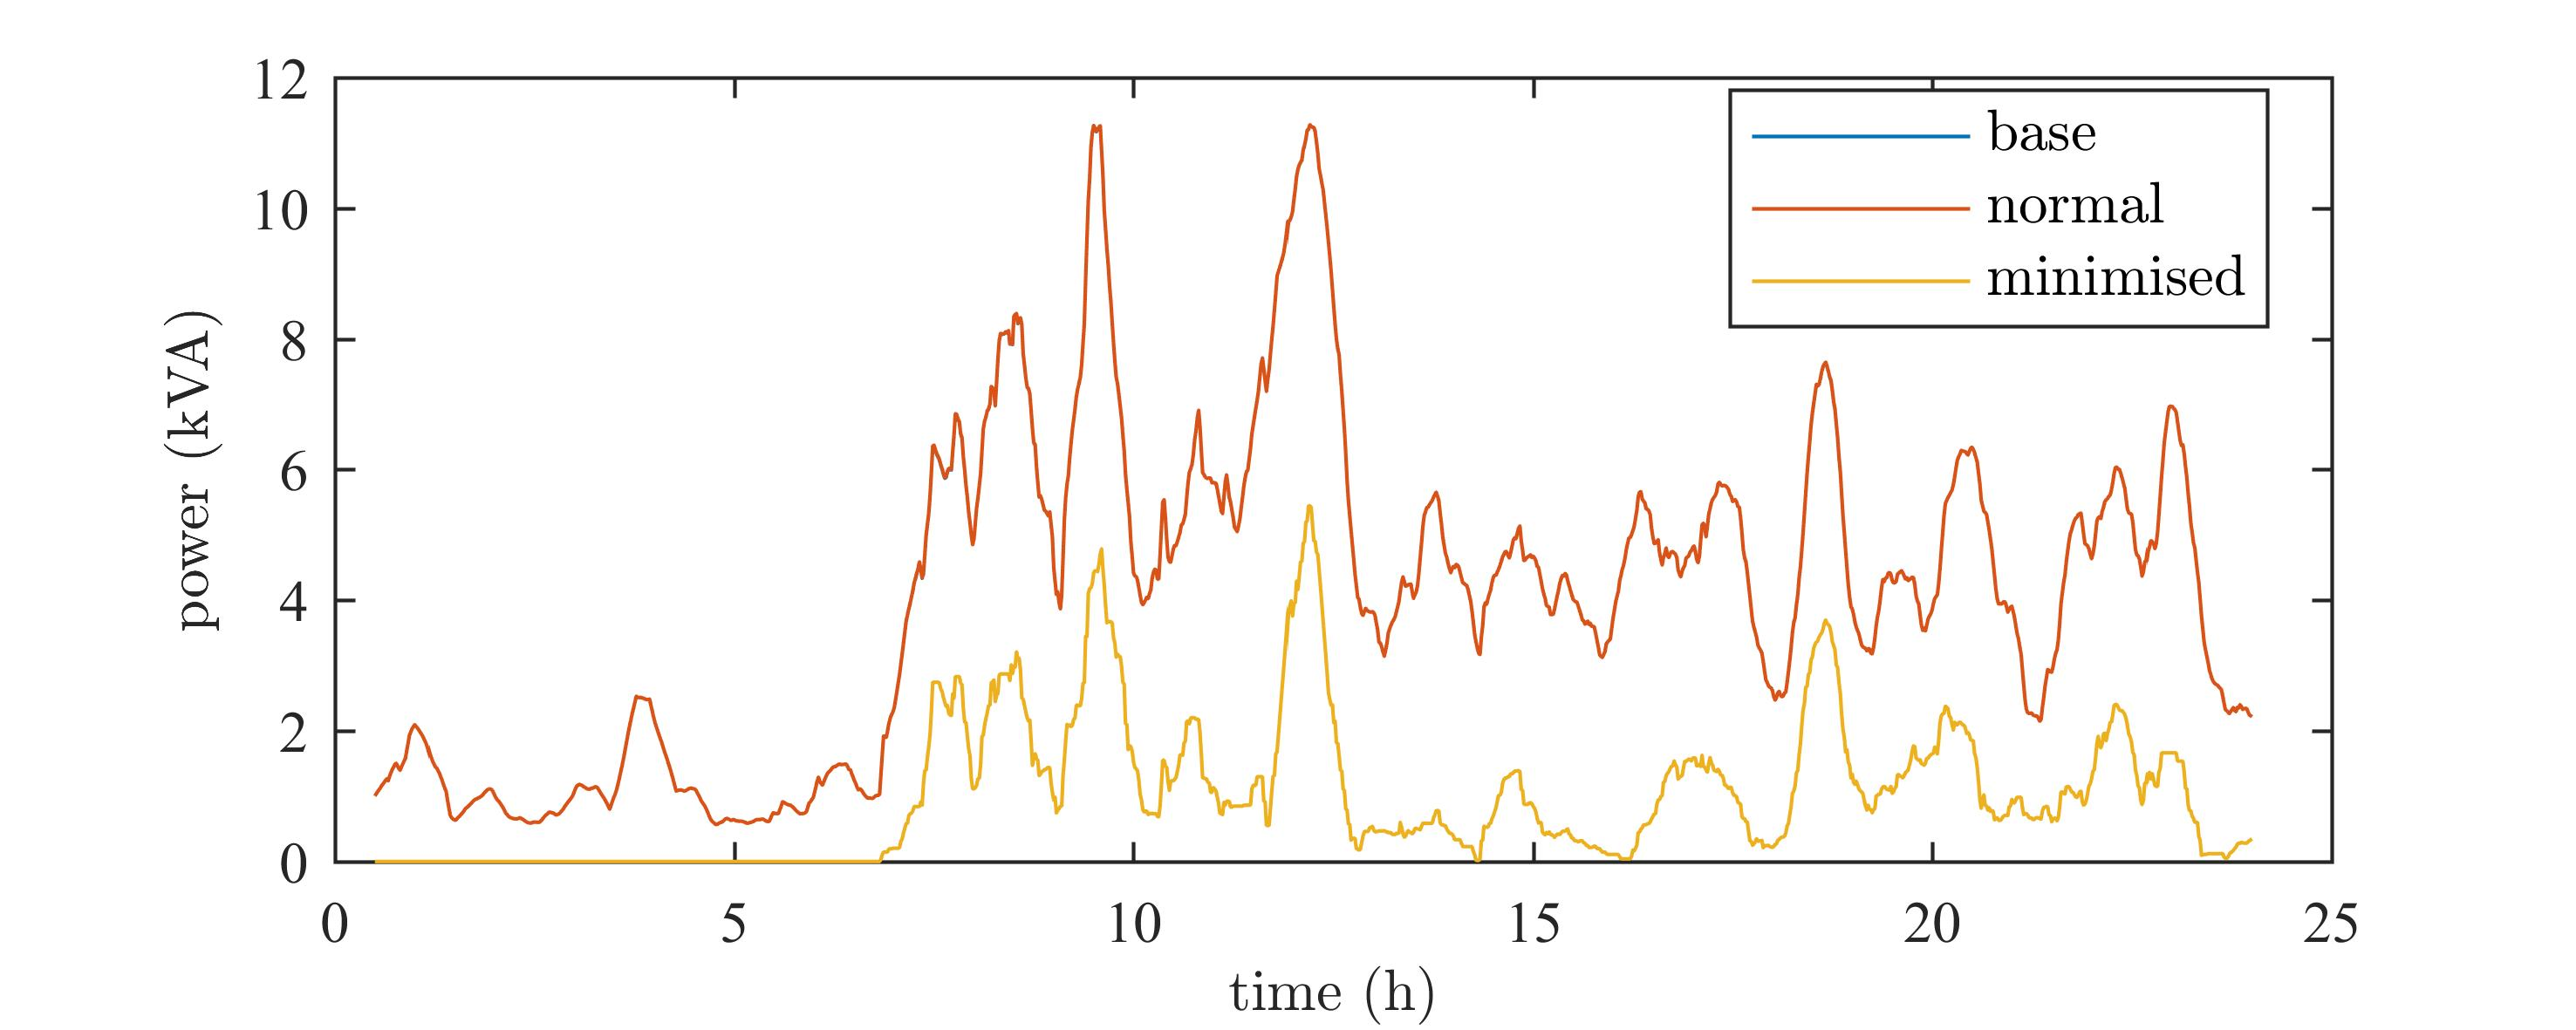
\includegraphics[width=\textwidth]{_chapter1/fig/ts-neutral-power-2}
\caption{Neutral power reduction due to the ESMU schedule adjustments}
\label{ch1:fig:ts-neutral-power}
\end{figure}

The results plotted in Figure \ref{ch1:fig:ts-neutral-power} show the network impact when adjusting the ESMU's schedule in order to minimise neutral power flow.
Incidentally, when applying the normal half-hourly ESMU schedule, neutral power is not affected at all.
The reason behind this was the choice of evenly assigning the scheduled power to all three phases, instead of taking into account the phases' loadings.
Power factor on the other hand was impacted just by introducing the half-hourly ESMU schedule, as shown in the following figure.

\begin{figure}\centering
	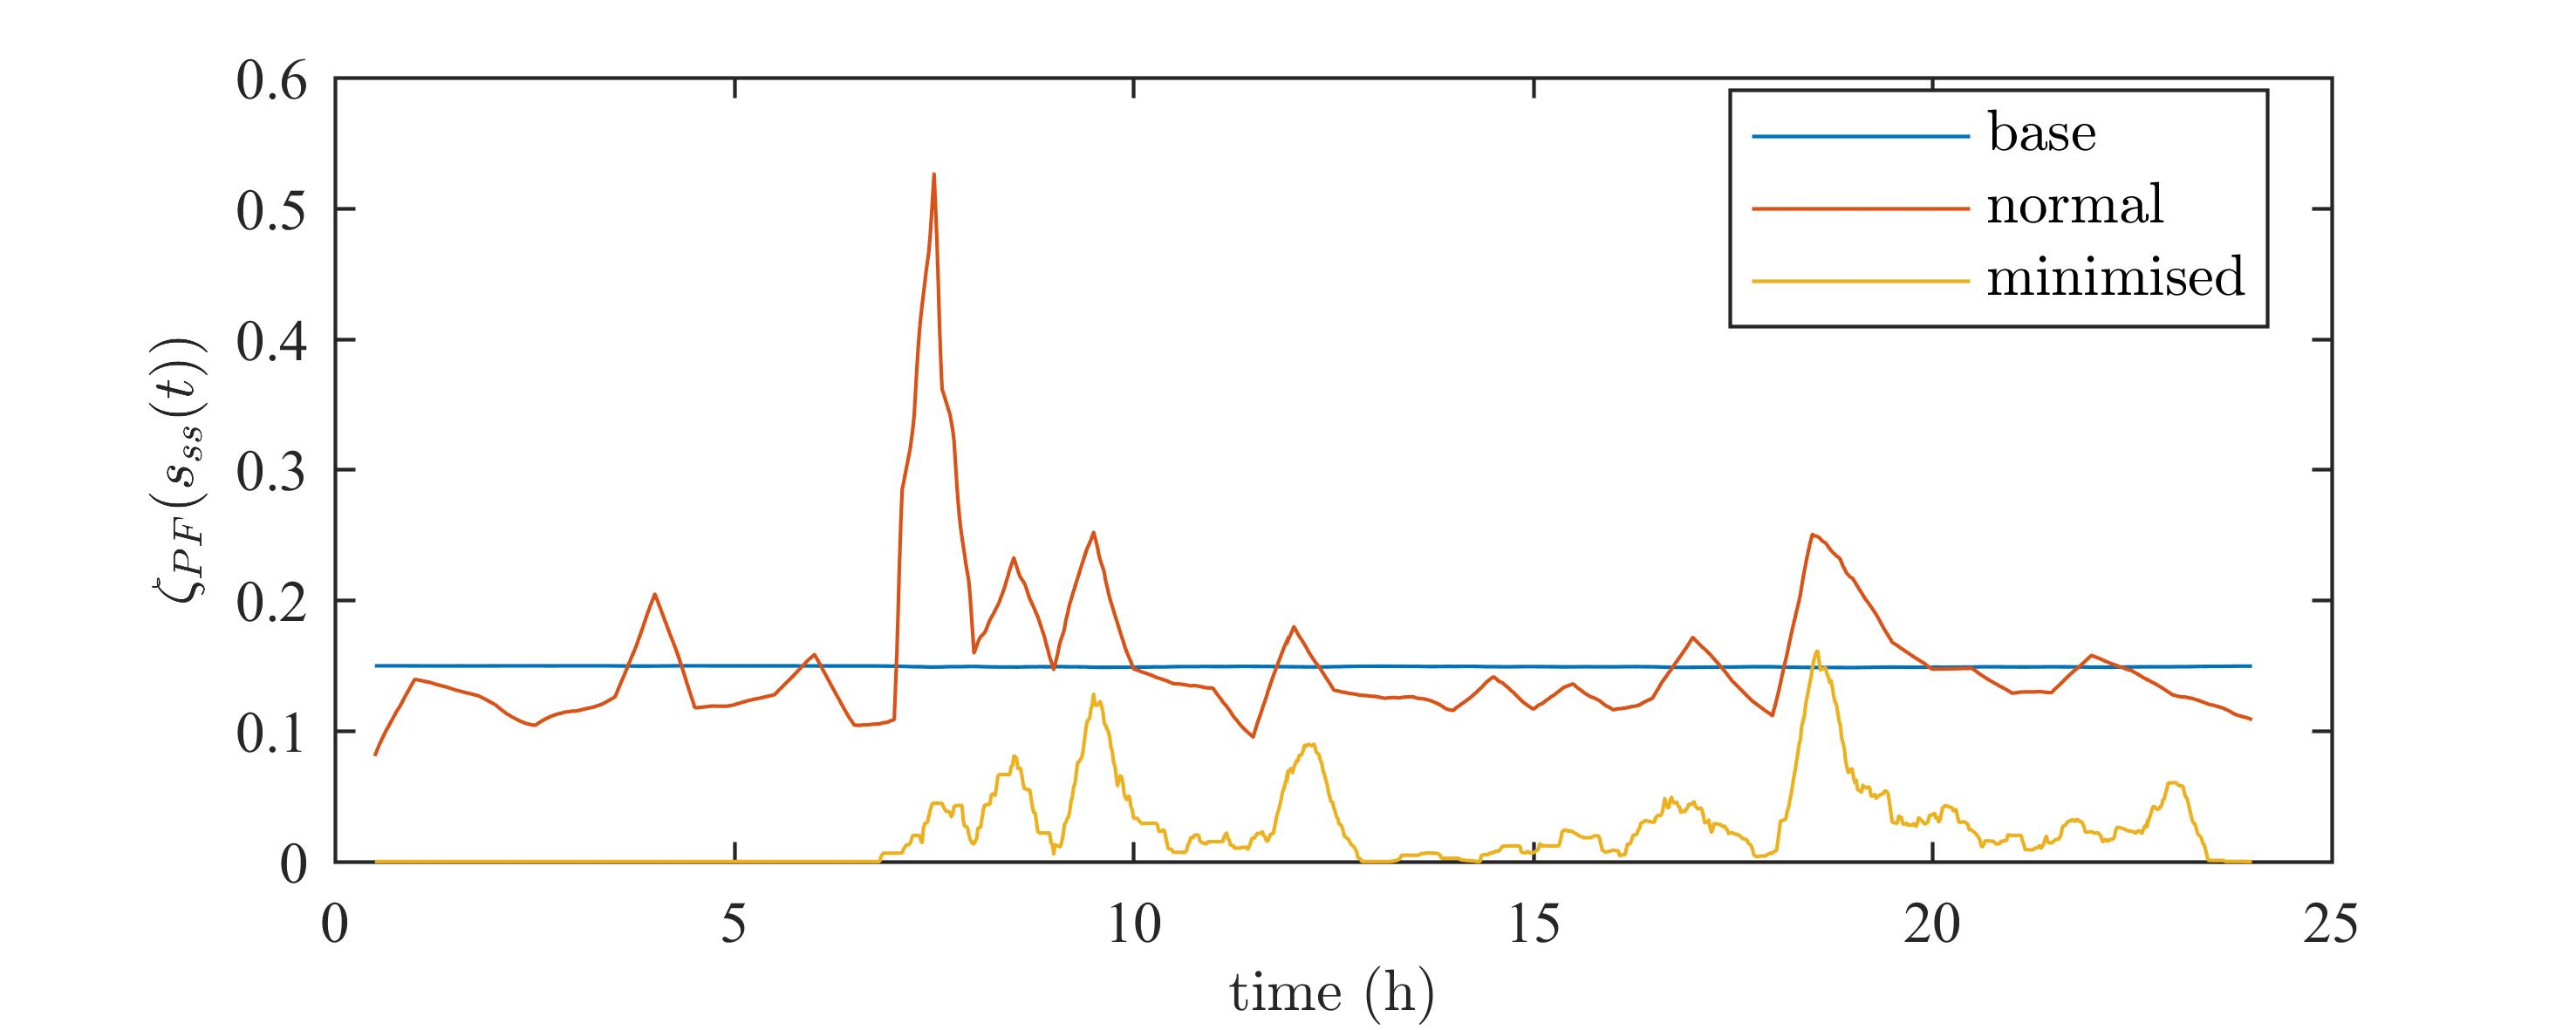
\includegraphics[width=\textwidth]{_chapter1/fig/ts-power-factor}
\caption{Power factor cost improvements due to the adjustment of the ESMU schedule}
\label{ch1:fig:ts-power-factor}
\end{figure}

Here, in Figure \ref{ch1:fig:ts-power-factor}, the power factor cost is successfully reduced during the entire day, in comparison to the normal cases.
In contrast, the base case had a constant power factor cost, due to aforementioned assignment of a constant power factor of 0.95 to all loads.
In reality, however, any network's power factor varies over time since the number of inductive machines and their associated inductive load varies constantly.
Nonetheless, the results would be similar but more variable when applied to a network with varying power factor, since the aim when adjusting the ESMU schedule was to reduce the power factor's deviation from unit power factor.
The final parameter that indicates system efficiency are the distribution losses.

\begin{figure}\centering
	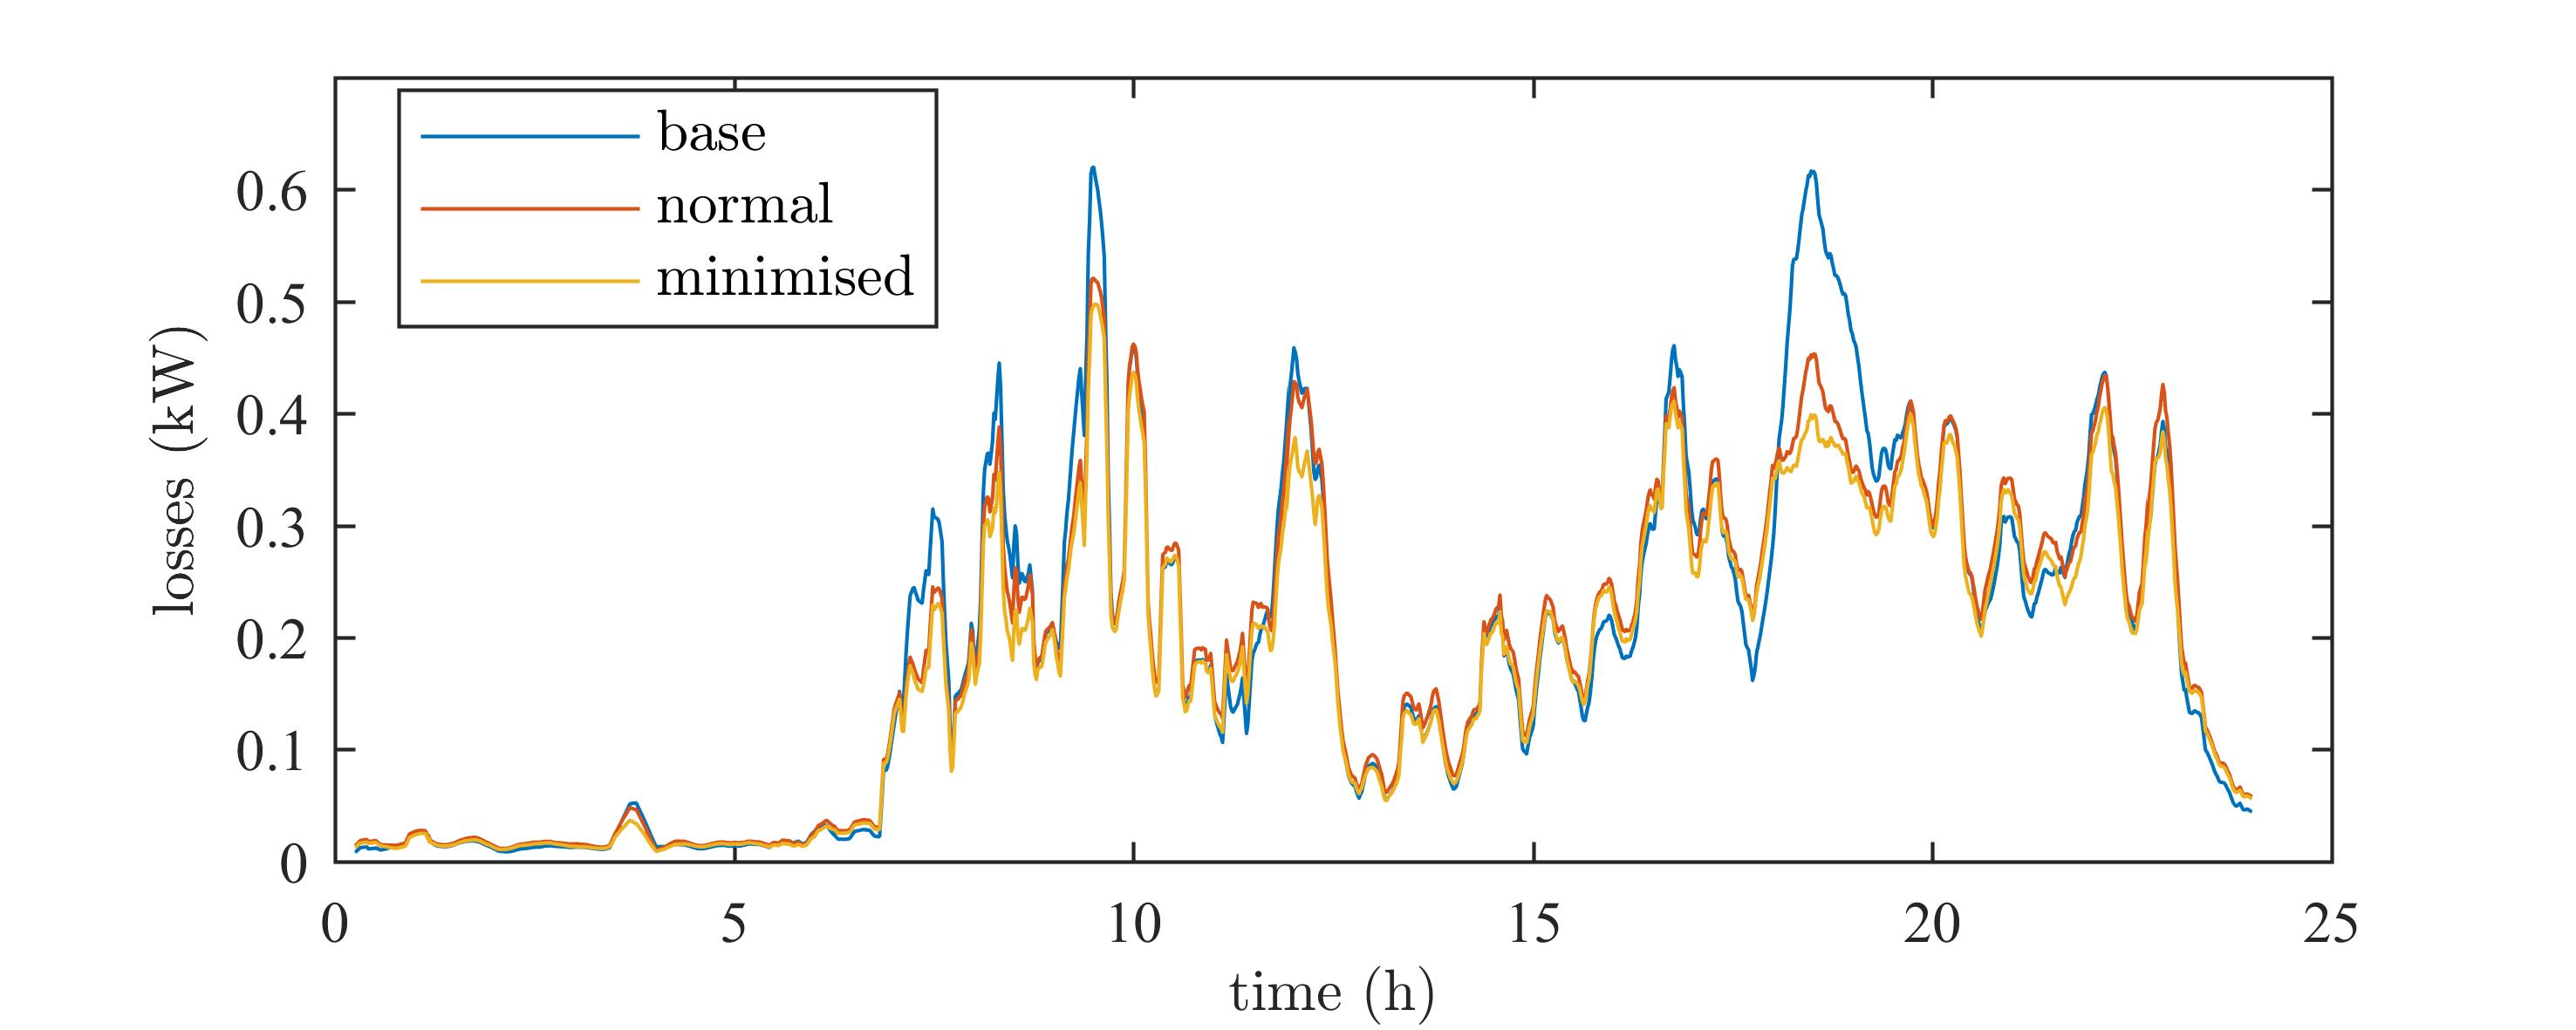
\includegraphics{_chapter1/fig/results/ts-losses_}
\caption{Instantaneous losses of the distribution network when adjusting the ESMU schedule in order to reduce the former \hl{(energy lost: 4.55kWh for base; 4.47kWh for normal; 4.19kWh for minimised)}.}
\label{ch1:fig:ts-losses}
\end{figure}

Figure \ref{ch1:fig:ts-losses} shows the reduction in distribution losses that were achieved when adjusting the ESMU schedule accordingly.
Again, the schedule adjustment reduced losses throughout the entire day.
In fact, an additional 6.42\% of energy savings could be achieved, simply by adjusting the ESMU's power injection and absorption behaviour.
Whilst this amount of energy may seem insignificant on a small scale, saving this amount of energy on a national level could potentially benefit the entire power network.
However, losses are difficult to measure and attempting to do so would most likely outweigh the benefits.

Instead, a better way of relieving stress from the power network is to minimise its assets utilisation by mitigating demand spikes.
Since the ESMU was constraint not to deviate from its underlying half-hourly schedule, only phase related demand differences could be addressed.
Those differences could however be addressed successfully, as shown in the following figure.

\begin{figure}\centering
	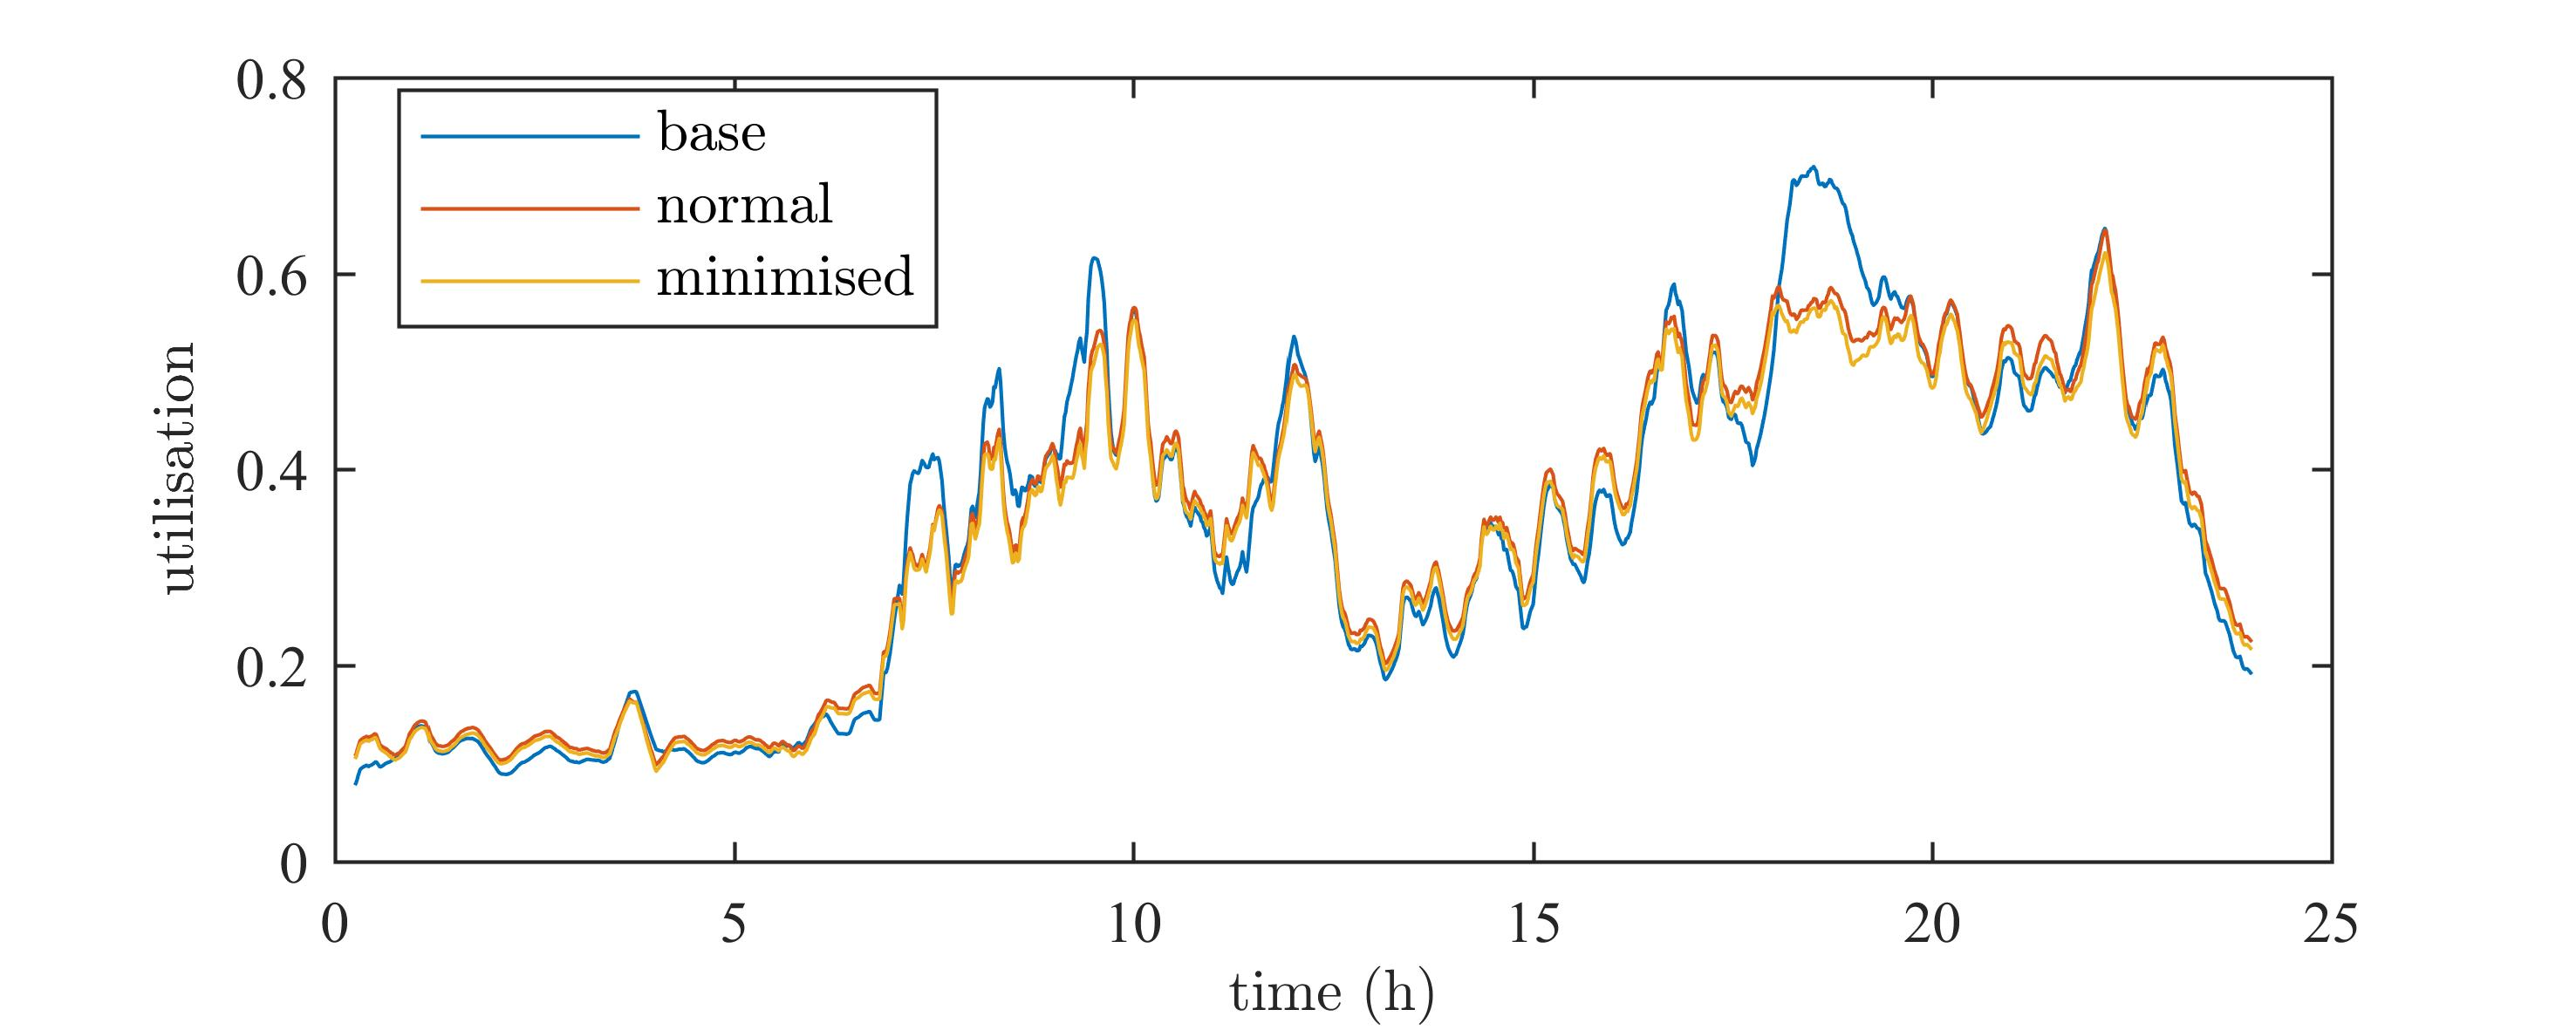
\includegraphics{_chapter1/fig/results/ts-all-line-utilisation_}
\caption{Improvement of the worst line utilisation across the entire network when adjusting the ESMU schedule correspondingly.}
\label{ch1:fig:ts-all-line-utilisation}
\end{figure}

Whilst the worst line utilisation is predominantly driven by the half-hourly charging and discharging behaviour of the ESMU, a subtle reduction could be achieved throughout the entire day, as shown in Figure \ref{ch1:fig:ts-all-line-utilisation}.
Yet as mentioned before, the constraint that is imposed due to the underlying half-hourly schedule significantly limits this improvement in network performance.

\subsection{Difference Analysis}
\label{ch1:subsec:difference-analysis}

In order to gage the whether the is a statistical difference in network performance, a box-plot was generated for each case.
The underlying data for each box-plot is the paired difference between the corresponding case's costs and the associated normal case's costs, i.e. when letting the ESMU operate normally, without adjusting its schedule.
Any positive difference in those costs indicates an improvement to the system's performance, whilst a negative difference would imply a worsening.

Here, the improvements for each individual cost are compared and plotted in Figure \ref{ch1:fig:boxplot-overall-improvements}.
A further set of comparing figures is also included in Appendix Section \ref{appx-a:ch1:additional-difference-analysis}, where the impacts on all costs, when minimising a for only an individual cost are compared.
Instead of including all these figures in the main body of this Thesis, the sum of all costs is computed and included in a table to give a more comprehensive indication of these so called cross-cost improvements.

\begin{figure}\centering
	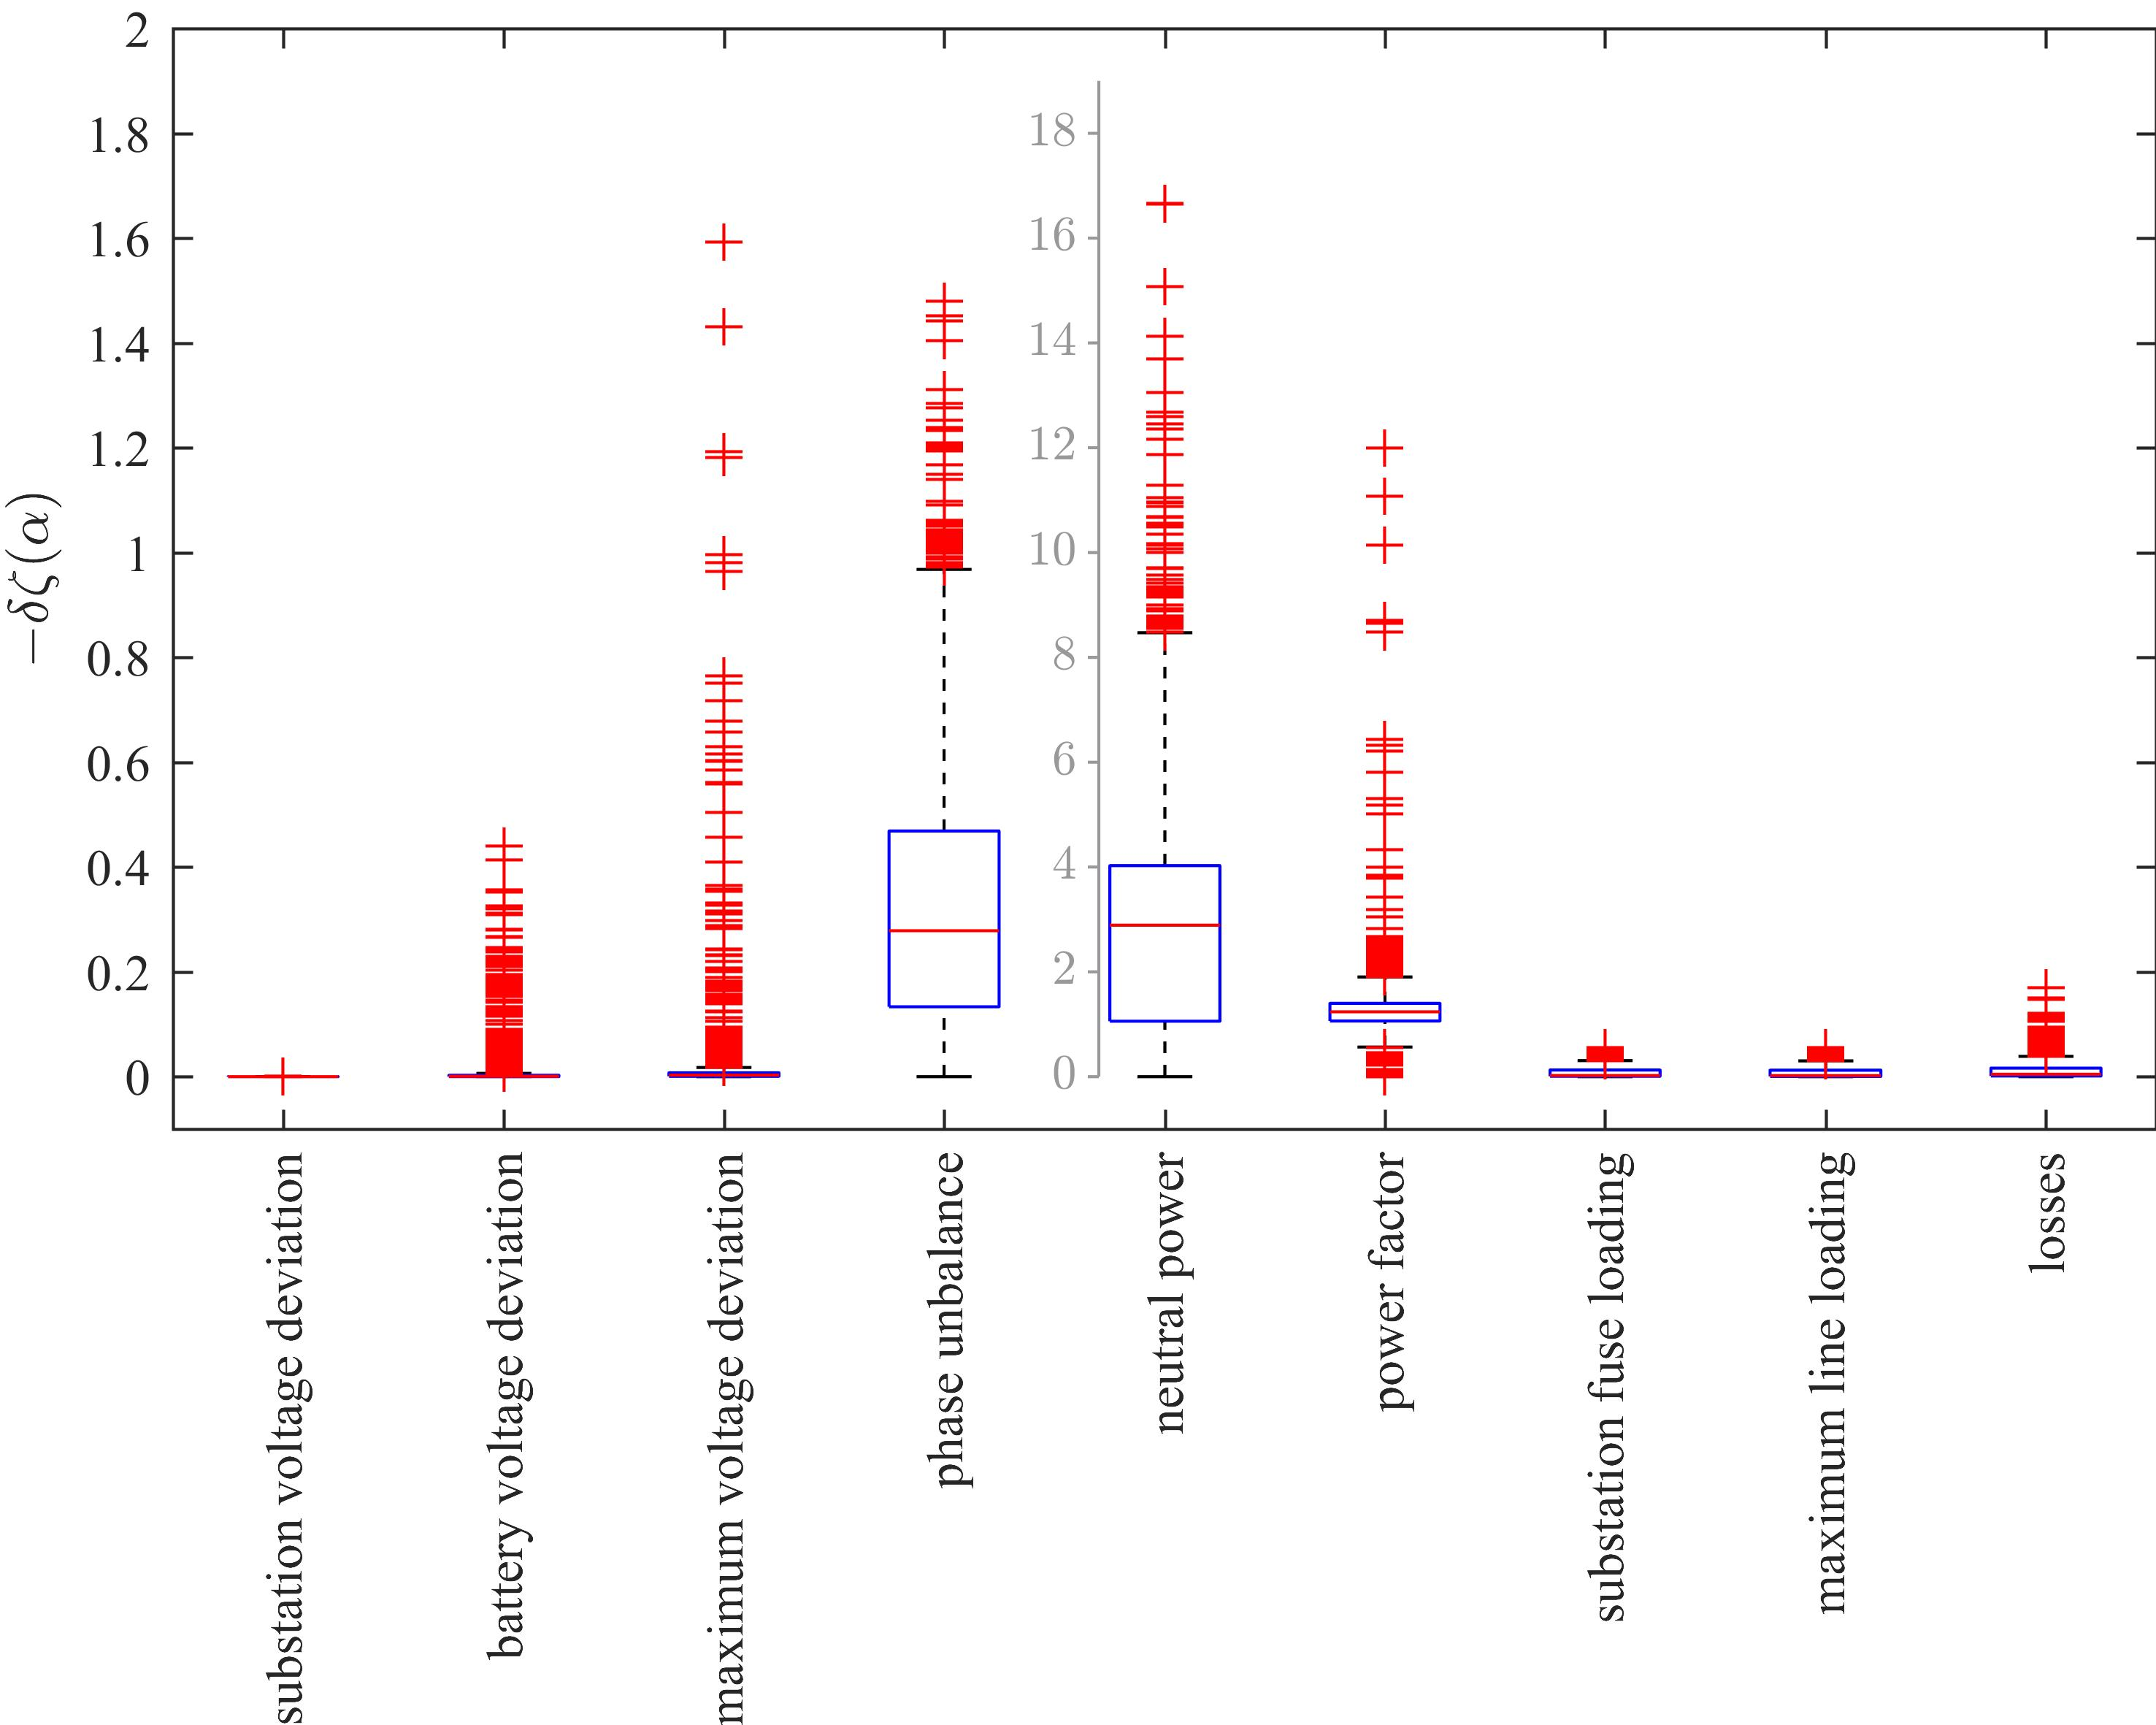
\includegraphics[width=\textwidth]{_chapter1/fig/results/boxplot-overall-improvements}
\caption{Cost-function improvement spread, when comparing against the normal ESMU operation case and when optimising for the underlying cost (a separate y-axis is introduced for the optimisation of ``neutral power'').}
\label{ch1:fig:boxplot-overall-improvements}
\end{figure}

In Figure \ref{ch1:fig:boxplot-overall-improvements}, it can be seen that the most significant cost related impact on the network was on the improvement of phase unbalance, neutral power and power factor.
The reason for this noticeably larger impact is that the ESMU can assign its scheduled active power in an arbitrary manner to all three phases, as long as the predetermined half-hourly schedule is followed.
It is this constraint of having to obey the schedule, that limits the impact on all other key network parameters.
Reactive power on the other hand is not directly limited to this constraint, since it is not scheduled as such.
The only limit that applies to the ESMU's reactive power injection capabilities, is the remaining PMU capacities when applying the active powers in order to follow the half-hourly schedule.
Also, unlike active power, reactive power has a smaller impact on the LV network due to its physical property, i.e. being more resistive than inductive.
Nonetheless, all key network parameters were impacted positively when they became subject to their associated cost-function minimisation.

To summarise the aforementioned cross-cost improvements (which are presented in detail in the Appendix, Section \ref{appx-a:ch1:additional-difference-analysis}), all costs are calculated for all minimisation cases, compared against the normal case, and accumulated into a single value.
This value is defined as the ``cumulative cost difference''.
Additionally, the normal case is compared to the base case in a similar manner.
This was done since it is interesting to see how the half-hourly schedule impacted the network.

\begin{sidewaystable}\centering
\definecolor{light_blue}{rgb}{0.9, 0.9, 1.0}
\definecolor{dark_blue}{rgb}{0.5, 0.5, 1.0}
\begin{tabular}{cc|ccccccccc|}
& & \multicolumn{9}{c}{minimisation cases} \\
& \rotatebox[origin=l]{90}{normal}& \rotatebox[origin=l]{90}{substation voltage deviation}& \rotatebox[origin=l]{90}{battery voltage deviation}& \rotatebox[origin=l]{90}{maximum voltage deviation}& \rotatebox[origin=l]{90}{phase unbalance}& \rotatebox[origin=l]{90}{neutral power}& \rotatebox[origin=l]{90}{power factor}& \rotatebox[origin=l]{90}{substation fuse loading}& \rotatebox[origin=l]{90}{maximum line loading}& \rotatebox[origin=l]{90}{losses} \\
\hline
\multicolumn{1}{r|}{substation voltage deviation} & 0.00 & \cellcolor{light_blue}0.08 & -2.49 & -1.39 & -4.89 & -8.72 & \cellcolor{light_blue}0.04 & 0.00 & \cellcolor{light_blue}0.01 & -1.09 \\
\multicolumn{1}{r|}{battery voltage deviation} & -5.01 & -0.40 & \cellcolor{light_blue}15.52 & \cellcolor{light_blue}17.04 & \cellcolor{light_blue}9.14 & \cellcolor{light_blue}14.93 & -2.85 & -0.43 & -1.62 & \cellcolor{light_blue}13.69 \\
\multicolumn{1}{r|}{maximum voltage deviation} & -6.83 & -1.15 & \cellcolor{light_blue}28.22 & \cellcolor{light_blue}36.42 & \cellcolor{light_blue}24.66 & \cellcolor{light_blue}33.05 & -3.07 & -0.56 & -2.57 & \cellcolor{light_blue}25.44 \\
\multicolumn{1}{r|}{phase unbalance} & \cellcolor{light_blue}12.15 & \cellcolor{light_blue}40.93 & \cellcolor{light_blue}284.87 & \cellcolor{light_blue}380.57 & \cellcolor{light_blue}490.22 & \cellcolor{light_blue}351.35 & \cellcolor{light_blue}40.66 & \cellcolor{light_blue}10.02 & \cellcolor{light_blue}5.03 & \cellcolor{light_blue}441.24 \\
\multicolumn{1}{r|}{neutral power} & -0.83 & -96.72 & \cellcolor{light_blue}2303.70 & \cellcolor{light_blue}1642.37 & \cellcolor{light_blue}2698.78 & \cellcolor{light_blue}4415.85 & \cellcolor{light_blue}319.23 & \cellcolor{light_blue}133.46 & \cellcolor{light_blue}53.53 & \cellcolor{light_blue}2401.12 \\
\multicolumn{1}{r|}{power factor} & -0.27 & \cellcolor{light_blue}159.42 & -7.63 & -37.25 & -633.30 & -314.11 & \cellcolor{light_blue}183.01 & \cellcolor{light_blue}145.35 & \cellcolor{light_blue}136.87 & \cellcolor{light_blue}88.84 \\
\multicolumn{1}{r|}{substation fuse loading} & \cellcolor{light_blue}5.14 & \cellcolor{light_blue}13.34 & -0.43 & -8.69 & -51.76 & -72.68 & \cellcolor{light_blue}14.37 & \cellcolor{light_blue}10.98 & \cellcolor{light_blue}10.91 & \cellcolor{light_blue}5.64 \\
\multicolumn{1}{r|}{maximum line loading} & \cellcolor{light_blue}4.53 & \cellcolor{light_blue}12.88 & -6.17 & -10.04 & -80.41 & -97.30 & \cellcolor{light_blue}13.89 & \cellcolor{light_blue}10.69 & \cellcolor{light_blue}10.94 & \cellcolor{light_blue}4.72 \\
\multicolumn{1}{r|}{losses} & \cellcolor{light_blue}4.34 & \cellcolor{light_blue}7.22 & \cellcolor{light_blue}13.38 & -4.46 & -46.37 & -66.32 & \cellcolor{light_blue}12.89 & \cellcolor{light_blue}9.65 & \cellcolor{light_blue}9.02 & \cellcolor{light_blue}17.13 \\
\end{tabular}
\caption{Cross-cost improvements due to adjustments to the original ESMU schedule.}
\label{ch1:tab:cost-table}
\end{sidewaystable}


The cumulative cost differences are tabulated in Table \ref{ch1:tab:cost-table}.
Every improvement in system operation is reflected as a reduction in cost, when compared to the corresponding normal or base case.
Therefore, a positive cumulative cost difference indicates, that over an entire day, the system operation improved in regards to the given cost.
Here, these improvements, i.e. positive cumulative cost differences, have been highlighted.

As expected, all entries along the diagonal, i.e. where the evaluated cost is also the cost that was minimised for the underlying case, nearly always show the largest cumulative cost differences.
It is also interesting to see, how a specific cost minimisation had noticeable impacts on different cumulative cost measures.
For example, adjusting the ESMU schedule to achieve the largest reduction in distribution losses (i.e. far right column) had an impact on all key network parameters.
This impact was also positive in nature for all key network parameters (apart from substation voltage deviation).

Then again, although the network optimisation for an optimised line and fuse loading did result in a positive cumulative cost difference, reduction in power factor had a more significant positive impact.
The reason behind this is that instantaneous apparent power contributes to the loading.
This means, that increasing the power factor inadvertently reduces reactive load, which in turn lowers the total current flowing into the system.
Not knowing what cost to address first, makes it difficult for the used solving algorithm to find the global minimum.
To improve the performance of the adjusted ESMU schedule, one could concatenate the cost minimisation in series to locate regions where lower minima may be found.
In this case at least, maximising the network's power factor before addressing fuse and line utilisation would have been a better choice.

\subsection{Probability Density Analysis}
\label{ch1:subsec:probability-density-analysis}

The final part of analysing the results is to statistically determine, whether the cumulative cost differences are indeed significantly different.
To do so, the probability density functions (PDF) of the  cost differences is analysed using a null hypothesis test.
However, the underlying data had to be conditioned in order to meet all prerequisites that are necessary to perform a null hypothesis test, such as the standard $t$-test.
These prerequisites include stationarity, low auto-correlation and high gaussianity of the underlying time-series.
The conditioning to meet such these prerequisites had to be carried out without falsifying the data, therefore limiting possible operations to time-series division and linear transformations.
Details on the exact steps are outside the scope of this chapter, yet have been included in the appendix for completeness.

\begin{sidewaystable}\centering
\definecolor{light_blue}{rgb}{0.9, 0.9, 1.0}
\definecolor{dark_blue}{rgb}{0.5, 0.5, 1.0}
\definecolor{light_red}{rgb}{1.0, 0.5, 0.5}
\begin{tabular}{cc|ccccccccc|}
& & \multicolumn{9}{c}{minimisation cases} \\
& \rotatebox[origin=l]{90}{normal}& \rotatebox[origin=l]{90}{substation voltage deviation}& \rotatebox[origin=l]{90}{battery voltage deviation}& \rotatebox[origin=l]{90}{maximum voltage deviation}& \rotatebox[origin=l]{90}{phase unbalance}& \rotatebox[origin=l]{90}{neutral power}& \rotatebox[origin=l]{90}{power factor}& \rotatebox[origin=l]{90}{substation fuse loading}& \rotatebox[origin=l]{90}{maximum line loading}& \rotatebox[origin=l]{90}{losses} \\
\hline
\multicolumn{1}{r|}{substation voltage deviation} & $0.851$ & \cellcolor{light_blue}$<0.001$ & $0.999$ & $1.000$ & $0.999$ & $1.000$ & \cellcolor{light_blue}$<0.001$ & \cellcolor{light_blue}$<0.001$ & \cellcolor{light_blue}$<0.001$ & $0.999$ \\
\multicolumn{1}{r|}{battery voltage deviation} & $0.899$ & \cellcolor{light_blue}$<0.001$ & \cellcolor{light_blue}$<0.001$ & \cellcolor{light_blue}$<0.001$ & \cellcolor{light_blue}$<0.001$ & \cellcolor{light_blue}$<0.001$ & \cellcolor{light_blue}$0.022$ & \cellcolor{light_blue}$0.018$ & $0.325$ & \cellcolor{light_blue}$<0.001$ \\
\multicolumn{1}{r|}{maximum voltage deviation} & $0.718$ & \cellcolor{light_blue}$0.000$ & \cellcolor{light_blue}$<0.001$ & \cellcolor{light_blue}$<0.001$ & \cellcolor{light_blue}$<0.001$ & \cellcolor{light_blue}$<0.001$ & $0.086$ & $0.167$ & $0.772$ & \cellcolor{light_blue}$<0.001$ \\
\multicolumn{1}{r|}{phase unbalance} & $0.331$ & \cellcolor{light_blue}$<0.001$ & \cellcolor{light_blue}$<0.001$ & \cellcolor{light_blue}$<0.001$ & \cellcolor{light_blue}$<0.001$ & \cellcolor{light_blue}$<0.001$ & \cellcolor{light_blue}$<0.001$ & \cellcolor{light_blue}$0.001$ & \cellcolor{light_blue}$0.038$ & \cellcolor{light_blue}$<0.001$ \\
\multicolumn{1}{r|}{neutral power} & $0.940$ & $0.999$ & \cellcolor{light_blue}$<0.001$ & \cellcolor{light_blue}$<0.001$ & \cellcolor{light_blue}$<0.001$ & \cellcolor{light_blue}$<0.001$ & \cellcolor{light_blue}$<0.001$ & \cellcolor{light_blue}$<0.001$ & \cellcolor{light_blue}$0.016$ & \cellcolor{light_blue}$<0.001$ \\
\multicolumn{1}{r|}{power factor} & $0.488$ & \cellcolor{light_blue}$<0.001$ & \cellcolor{light_blue}$0.020$ & $0.999$ & $0.999$ & $1.000$ & \cellcolor{light_blue}$<0.001$ & \cellcolor{light_blue}$<0.001$ & \cellcolor{light_blue}$<0.001$ & \cellcolor{light_blue}$<0.001$ \\
\multicolumn{1}{r|}{substation fuse loading} & $0.777$ & \cellcolor{light_blue}$<0.001$ & $0.929$ & $0.999$ & $0.999$ & $1.000$ & \cellcolor{light_blue}$<0.001$ & \cellcolor{light_blue}$<0.001$ & \cellcolor{light_blue}$<0.001$ & \cellcolor{light_blue}$0.001$ \\
\multicolumn{1}{r|}{maximum line loading} & $0.846$ & \cellcolor{light_blue}$<0.001$ & $0.996$ & $0.999$ & $0.999$ & $0.999$ & \cellcolor{light_blue}$<0.001$ & \cellcolor{light_blue}$<0.001$ & \cellcolor{light_blue}$<0.001$ & $0.102$ \\
\multicolumn{1}{r|}{losses} & $0.881$ & \cellcolor{light_blue}$<0.001$ & \cellcolor{light_blue}$<0.001$ & $0.637$ & $0.910$ & $0.999$ & \cellcolor{light_blue}$<0.001$ & \cellcolor{light_blue}$<0.001$ & \cellcolor{light_blue}$<0.001$ & \cellcolor{light_blue}$<0.001$ \\
\end{tabular}
\caption{$p$-values for statistical evidence of cross-cost improvements based on statistical two-sample single-tailed $t$-test.}
\label{ch1:tab:t-test-table}
\end{sidewaystable}


Table \ref{ch1:tab:t-test-table} presents the results from this analysis.
Here, $p$-values have been tabulated and those cells with a value below $0.05$ are highlighted in blue.
A similar pattern to that in the previous table seen, where the cumulative cost difference was tabulated.
Here however, instead of just comparing costs, statistical indications to support the significance of the findings is presented, here.
In combination with the preceding table, one can determine that e.g. the impact of optimising operation based on maximum voltage deviation has little to no significant impact on improvements in power factor.
The most critical finding is however, that each cost minimisation did indeed result in significant improvement of corresponding network operation.
